\chapter{Chopping}
\label{ch:chopping}
\todo{Better headline}

\subsection*{General idea and length}
\begin{itemize}
	\item Explain the problem (want to do chopping, but current setup is too slow and limited by rise times) (1 page)
	\item Give solution which is EOMs (1 page)
	\item Give theory behind eoms (length as is)
	\item Give experimental results of the two pockels cells that were tested (because we are finding the extinction ratio, I should also give an error and maybe implement the other fit (sign(sin(x))) (maybe 1-2 pages longer).
\end{itemize}
Maybe the problem (chopping can be better) could be written in its own section and explained in more detail.
\todo{chapter start}

In the experiment, optical tweezers are used to generate two-dimensional arrays of single atoms. By using optical tweezers, each atom can be addressed individually and therefore parameters such as inter-atomic distances and trap depths can be adjusted freely. In order to load atoms into the optical tweezers, they have to undergo some cooling stages first. Being vaporized from a solid sample of \ce{^{39}K}, the atoms move towards the center of a vacuum chamber through a Zeeman slower. The slower cools the atoms longitudinally, after which they are trapped and compressed in a \ac{mot}. Cooling is done in a gray molasses on the D1-line, after which the atoms will be loaded into the tweezers. However, loading directly from the gray molasses proves difficult, due to the large light shifts of the D1 excited state, making it highly anti-trapped. To overcome this issue, trapping and cooling beams can be alternated \cite{Hutzler2017}. By having the frequency of alternating the beams much larger than the trapping frequency, the atoms see an effective, averaged, trap. This way, they don't scatter near-resonant photons, effectively eliminating light shifts.

So far, alternating between molasses cooling and trapping light, called chopping, was achieved using an \ac{aom}. However, the switching speed in an \ac{aom} is limited by the speed of sound in the medium (here, TeO2 has \SI{4.2}{\milli\meter\per\micro\second}) and results in a chopping frequency of $\SI{1.4}{\mega\hertz}$, governed by the \ac{aom} with the slowest rise time, which can be seen in Figure~\ref{fig:aom_chopping}. By increasing the chopping frequency, the atoms will heat less during each trapping cycle. However, more importantly, as the atoms only see an averaged trap given by the duty cycle of the trapping beam, more laser power can be used per tweezer if the beam remains on for a longer time. This also means, that more tweezers can be deployed and larger systems explored.
\todo{Why does it say Figure 3?}

\begin{figure}[t]
	\label{fig:aom_chopping}
\centering{%
	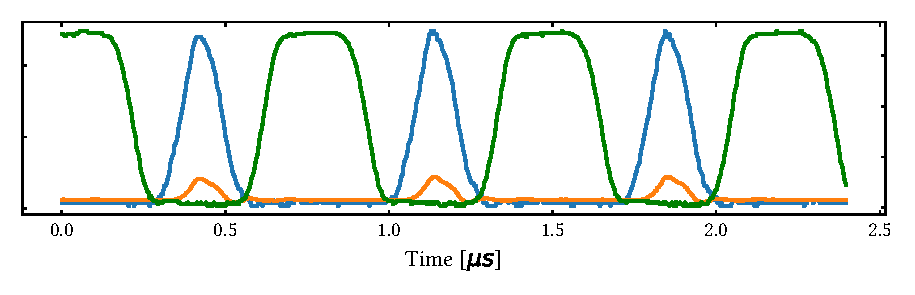
\includegraphics{figures/chopping_155.pdf}
	\caption{Chopping in the experiment. Laser beams alternate between each other, with blue being the MOT cooler, orange the MOT repumper and green the SLM tweezer. The amplitude of the MOT beams is limited due to the risetime of the \acp{aom}.}
}
\end{figure}
\todo{acronyms? MOT, SLM}
\todo{explain figure again}

Achieving larger duty cycles and higher chopping frequencies is possible by using \acp{eom}, which are not limited by acoustic waves. The optical medium is modulated using electric fields, and in fact, can be switched as fast as common condensators. Light entering the modulator will have its polarization turned, depending on the electric field that is applied. Therefore, in the following, polarization of electro-magnetic waves is discussed briefly, which is followed by the main effect governing the devices tested in this thesis - the pockels effect. The devices are then evaluated by filtering one polarization component and the rise times and extinction ratio measured. The new system will be able to switch with rise times on the order of nanoseconds, improving the current system by at least two orders of magnitude.

The devices tested in this thesis are both capable of switching on nanosecond scales, improving the current chopping rate by three orders of magnitude. The theory behind the linear electro-optical effect is discussed after a short recourse on polarization of electromagnetic waves. Lastly, experimental evaluations for two \acp{eom} are presented and discussed.

\todo{say something about that chopping reduces lifetime}


\section{Theory on Polarization}

\label{sec:pol}

Switching laser beams using \acp{eom} means turning and filtering the polarization of the light. Therefore in the following is discussed the theory behind polarized monochromatic electromagnetic waves, leading to the pockels effect governing \acp{eom}.

Polarization of electromagnetic waves is understood as the orientation of the wave in space, transverse to the direction of movement. In general, a wave travelling along the z-axis can be oriented somewhere in the x-y plane. Therefore, writing the electric field component of the light in this basis takes the following form:

\begin{equation}
	\mathbf{E}(\mathbf{x}, t) = E_x cos\left(kx - wt + \phi_x\right) \mathbf{e_x} + E_y cos\left(ky - wt + \phi_y\right) \mathbf{e_y}.
\end{equation}

Here, $k$ and $w$ refer to the wave number and frequency respectively.
Depending on the amplitudes $E_x$ and $E_y$ and the phases $\phi_x$ and $\phi_y$, the wave can be in different polarization states. If it is not possible to write the wave in this basis, the light is unpolarized. Otherwise, it is \textbf{linear}, when either one of the amplitudes $E_x$ or $E_y$ is zero or when the phase difference $\Delta \phi = \phi_x - \phi_y$ evaluates to 0 or $\pi$. It is \textbf{circular}, when the phase difference $\Delta \phi = \pm \pi/2$ and the amplitudes are the same, $E_x = E_y$. In any other case, the wave is \textbf{elliptically} polarized.

By changing the phases of the wave relative to each other therefore gives the ability to affect the polarization. Light traversing a medium will accumulate a phase shift, depending on the refractive index, which affects the speed of light in the medium. Therefore, media that have different refractive indices $n_x, n_y$ along the two axes $x$ and $y$ means changing the relative phases of the wave:

\begin{align}
	\label{eq:pol,phases}
	\phi_x(z) = k_0 n_x z \\
	\phi_y(z) = k_0 n_y z
\end{align}

where $k_0$ is the free space wave vector of the light. Then a device that retards the phase difference $\Delta \phi$ by $\pi/2$, which is a quarter of the wavelength, can change linearly polarized light to circularly polarized light (or vice-versa) and is therefore called a $\lambda / 4$ waveplate. Similarily, if the phase difference is changed by $\Delta \phi = \pi$, or a half wavelength, then we can turn linear polarization around a given axis or change the orientation of circularly polarized light. This is then called a $\lambda / 2$ waveplate. In the experiment, linearly polarized light will enter the \ac{eom}, which will act as a $\lambda / 2$ waveplate, turning the polarization by $\SI{90}{\degree}$, making it easy to filter unwanted polarization components and switching the light on and off.

\section{Electro-optical modulators}
\label{sec:eom}

Light travelling through a material generally has a speed smaller than the speed of light. This property of the material is the refractive index and is the ratio of the speed of light in the material to the speed of light in vacuum. Materials can change their refractive index by being exposed to an electric field, which in \acp{eom} is generally a crystal connected to two electrodes. There are two prominent electro-optical effects that need to be distinguished. If the refractive index changes linearly with the electric field, the effect is called Pockels effect and the \ac{eom} is called a pockels cell. The effect is discussed in the following and the pockels cells evaluated afterwards.

\subsection{Pockels effect}
\label{sec:pockels_effect}

As was motivated in the previous section, the goal of modulating light polarization is to change the relative refractive index of a medium in two axes. Following the argumentation from the book Fundamentals of Photonics \cite{Saleh1991}, the pockels effect can be found by evaluating the refractive index with respect to the electric field applied to the modulator. Writing this as $n(E)$ and applying a taylor expansion, we get the following expression:

\begin{equation}
	n(E) = n_0 + \frac{dn}{dE} E + \mathcal{O}(E^2)
\end{equation}

The pockels effect is the linear dependence of the refractive index to the electric field, therefore higher orders are neglected. The prefactor $dn / dE$ can be found from the change of electric impermeability $\Delta \eta$, which is the ability of a material to be penetrated by an electromagnetic field. From

\begin{align}
	\eta & = \frac{1}{n^2},
\end{align}
we get
\begin{align}
	\label{eq:pockel,refr}
	\Delta \eta = \frac{d \eta}{dn} \Delta n & = -\frac{2}{n_0^3} \frac{dn}{dE} E = \mathfrak{r} E.
\end{align}

This results in the quantity $\mathfrak{r} = -\frac{2}{n_0^3} \frac{dn}{dE}$, which is called the Pockels coefficient given in units of $\SI{}{\meter\per\volt}$. It can be measured by evaluating the refractive index of the material:

\begin{equation}
	n(E) = n_0 - \frac{1}{2} \mathfrak{r} n_0^3 E.
\end{equation}

As was seen in Equation~\ref{eq:pol,phases}, the refractive index directly affects the phase shift, which in turn changes the polarization of the light wave. Combining the results leads to an equation using parameters typically found in \acp{eom}:

\begin{align}
	\phi & = k_0 L n \\
		 & = k_0 L n_0 - \frac{k_0}{2} L \mathfrak{r} n_0^3 E \\
		 & = \phi_0 - \frac{k_0}{2} L \mathfrak{r} n_0^3 E \\
		 & = \phi_0 - \frac{\pi}{\lambda_0} L \mathfrak{r} n_0^3 E
\end{align}

where the relation $k_0 = 2 \pi / \lambda_0$ of the wave number was used.

The pockels cells in this application act as dynamic wave retarders, therefore with the results from Section~\ref{sec:pol}, we can tune the phase difference $\Delta \phi = \phi_x - \phi_y$ along the axes $x$ and $y$ by applying an electric field. With the correct parameters, the phase difference lets the \ac{eom} act as a $\lambda / 2$ or $\lambda / 4$ waveplate. The following relations will help find the main formula governing pockels cells, resulting in the voltage that needs to be applied to the \ac{eom} in order to turn the polarization a given amount.

Labeling the refractive index in two dimensions as:

\begin{align}
	n_x(E) = n_{0,x} - \frac{1}{2} \mathfrak{r}_x n_{0,x}^3 E \\
	n_y(E) = n_{0,y} - \frac{1}{2} \mathfrak{r}_y n_{0,y}^3 E
\end{align}

then the phase difference becomes:

\begin{align}
	\Delta \phi & = \phi_{0,x} - \phi_{0,y} - \frac{\pi}{\lambda_0} E L \left(\mathfrak{r}_x n_x^3 - \mathfrak{r}_y n_y^3\right) \\
	\Delta \phi & = \Delta \phi_{0} - \frac{\pi}{\lambda_0} E L \left(\mathfrak{r}_x n_x^3 - \mathfrak{r}_y n_y^3\right).
	\label{eq:eom_phase_diff}
\end{align}

\begin{figure}[t]
\centering{%
	\import{figures}{eom_schematic.pdf_tex}
	\caption{Schematic view of light passing through an \ac{eom} of length $L$. The electrodes are positioned on the front and back side of the modulator, the same faces the light enters and exits. The light exiting the \ac{eom} has a relative phase shift $\Delta \Phi$ depending on the change of refractive index due to the applied voltage $V$.}
\label{fig:eom_schem}
}
\end{figure}

The next step is to replace the electric field by a voltage that can be applied to the pockels cell. For this, two electrodes are connected to the \ac{eom}, separated by a distance $d$. This gives the electric field as $E=V/d$. This quantity is replaced into Equation~\ref{eq:eom_phase_diff} and by realizing that the phase is unitless, all other prefactors of the voltage can be combined into one quantity, called the half-wave voltage $V_\pi$:

\begin{align}
	V_\pi = \frac{d}{L} \frac{\lambda_0}{\mathfrak{r}_x n_x^3 - \mathfrak{r}_y n_y^3}.
\end{align}

Thus, the phase difference can be rewritten as:

\begin{align}
	\label{eq:eom_phase_diff}
	\Delta \phi = \Delta \phi_0 - \pi \frac{V}{V_\pi}.
\end{align}

With this it is clear, that applying the voltage $V_\pi$, the pockels cell will act as a lambda-half waveplate. A visual represantation of the modulator and the light passing through it is given in Figure~\ref{fig:eom_schem}, highlighting the change in relative phase of the two components of the electro-magnetic wave.

We have seen, how applying a voltage to an electro-optical medium changes the refractive index and therefore affects the phase of an electromagnetic wave. By having two refractive indices in two axes, whose relative change depends on the applied voltage, it is therefore possible to modify the circularity and linearity of the polarization in an \acl{eom}.

\subsection{Driving a pockels cell}

With an understanding of the pockels effect governing the \acp{eom} tested in this thesis, it is now required to have electronics controlling voltages on the pockels cell. Having good electronics is important, as using pockels cells for switching of laser light means that rise and fall times are a direct consequence of the switching electronics used to apply the respective voltages to the pockels cell. However, materials suitable for use as \acp{eom}, such as \ac{bbo} and \ac{rtp} have half-wave voltages in the kilovolt-regime, meaning not only does the hardware need to be able to handle high voltages, but it is also necessary to switch the voltages on a fast timescale. This will turn out the be on the order of nanoseconds for the drivers used here (by BME Bergmann).

%When using \acp{eom} for switching of laser light, rise and fall times are a direct consequence of the electronics used to apply the respective voltages to the pockels cell. 
%Rise and fall times of pockels cells can go as low as nanoseconds. To make use of this speed, one has to deploy clever ways to drive the voltages, especially when these potentials are in the kilovolt-regime. For the two Pockels cells discussed in this thesis, specialized drivers by BME-Bergmann were used.

The pockels cell drivers discussed in the following contain the switching electronics necessary to drive the \acp{eom}. Moreover, it contains viewports for the laser light, such that the pockels cell can be integrated into the driver to not expose the high voltage to any parts of the experiment but the modulators. \todo{pic of driver in appendix and ref}The driver has an input for the high voltage and option for watercooling in order to compensate temperature instabilities on the pockels cell. Furthermore, it contains four inputs, in order to have full control over the switching of the voltages. These inputs are connected via SMB-connectors to any pulse synthesizers, such as waveform generators or delay cards and require TTL signals to operate switches inside the driver.

Therefore, it is necessary to understand the switching logic used inside the driver, in order to correctly drive the pockels cell and therefore turn the polarization of the light. Schematically, the driver is divided into the four switches mentioned above, that are controlled from the user: ON A, ON B, OFF A and OFF B. Two switches are connected to either side of the pockels cell, so A controls one electrode and B the other. Most importantly, the ON X and OFF X (X referring to either A or B) switches work exclusively, so sending a high to ON X will also send a low to OFF X and vice-versa. It is then possible to apply either a positive high voltage or a negative high voltage, depending on the state of the switches. For full identification of the circuit, which is given in Figure~\ref{fig:eom_driver_switches}, the side containing the positive voltage information is called high side and similarily the side containing the negative voltage information is called low side. The figure shows switching logics for two different drives used in the experiment. These are named by the manufacturer as dpp-type and bpp-type.

\begin{figure}[t]
\label{fig:eom_driver_switches}
\centering{%
	\begin{multicols}{2}
	\import{figures}{bpp_switches.pdf_tex}
	\import{figures}{dpp_switches.pdf_tex}
	\end{multicols}
	\caption{Schematic of the high voltage switches used inside the bpp-type (left) and dpp-type (right) pockels cell driver from BME Bergmann. Not-Gates on both A and B sides ensure that there is always a potential over the pockels cell. The blue and red paths indicate the connection to apply a positive and negative voltage over the pockels cell respectively.}
}
\end{figure}

A requirement for our experiment is to have the \acp{eom} work consistently. This means it is preferrable to only apply one type of voltage, because it can not be guaranteed that applying the same voltage with different polarity results in the same shift in polarization. This is due to the high fidelity of the pockels cell with respect to the input polarization and therefore highly depends on the alignment of the pockels cell. The diagram in Figure~\ref{fig:eom_timings} shows pulses applied to the switches on the A and B side, necessary to only drive positive voltages to the pockels cell.

For the bpp-type driver, this is straightforward, as closing high side A and low side B gives a positive voltage across the \ac{eom} and the inverse connects ground to ground through the \ac{eom}, giving zero voltage. The dpp-type driver on the other hand, has high and low voltages on either side of the pockels cell. Therefore, the sequence that results in positive and then no voltage across the \ac{eom} is, to close high side A and low side B switch, resulting in a positive voltage across the \ac{eom}. Afterwards, connecting high side A and high side B gives the same voltage on either side of the pockels cell, resulting in a net zero voltage. After this point, low side B is closed again, giving the same state as before. In the timing diagram, the low side A switch would be closed at this point. It is possible to keep high side A closed the entire time, however it is recommended in the documentation to alternate both switches in order to relax their states.

\begin{figure}[t]
\centering{%
	\import{figures}{bpp_timings.pdf_tex}
	\caption{Timing diagrams for the pockels cell drivers to turn the polarization of the \ac{eom} $\SI{90}{\degree}$. To get a positive high voltage from the bpp-type driver, the A and B side ON/OFF switches are flipped simultaneously. The dpp-type driver is more flexible, since it also allows negative voltages. The timings displayed here are an example to only apply positive voltages across the pockels cell.}
\label{fig:eom_timings}
}
\end{figure}

\subsection{Evaluation of Leysop Pockels cells}

In the following is discussed two pockels cells (from Leysop Ltd.). The \acp{eom} in contrast to the \acp{aom} in the current setup allow for longer duty cycles for the tweezer light. This means, the laser light needs to be switched on and off, which is achieved in pockels cells by exploiting the fact, that linearly polarized light can be filtered out. This is best achieved by placing a \ac{pbs} directly after the modulator as seen in Figure~\ref{fig:eom_setup}. This way, the setup can be configured such that applying no voltage means light passes through the beam splitter, while applying $V_\pi$ means the light gets reflected $\SI{90}{\degree}$ off the beam splitter, save for a fraction of light, given by the extinction ratio of the beam splitter (typically for the ones used in the experiment, the extinction ratio is about 200:1).

\begin{figure}[t]
	\label{fig:eom_setup}
\centering{%
	\import{figures}{eom_setup.pdf_tex}
	\caption{The efficiency of the \acp{eom} were evaluated by setting the polarization of the incoming light either horizontal or vertical using the waveplate. The pockels cell will then periodically turn the polarization $\SI{90}{\degree}$, which can be seen by measuring the voltage on the photodiode.}
\label{fig:eom_timings}
}
\end{figure}

Two  pockels cells were characterized by placing a photodiode on one end of the beam splitter. The \acp{eom} are labeled by the material of their nonlinear crystal, \ac{rtp} and \ac{bbo}. Their characteristics are summarized in Table~\ref{tbl:eom_crystals}, where half wave voltage is given for $\SI{1064}{\nano\meter}$ light. Both \acp{eom} are used in the chopping discussed earlier, where the \ac{rtp} crystal will be used for the $\SI{770}{\nano\meter}$. Consequently, \ac{bbo} will be for the $\SI{1064}{\nano\meter}$ tweezer light.
\todo{dont like this paragraph}

\begin{table}
\label{tbl:eom_crystals}
\centering
\begin{tabular}{l|l|l}
	\hline \hline
                                                                                     & RTP                                       & BBO \\ \thickhline
Aperture (crystal dimensions)                                                        & $\SI{3}{\milli\meter}$                    & $\SI{3}{\milli\meter}$   \\ \hline
Total crystal length (2 crystals)                                                    & $\SI{30}{\milli\meter}$                   & $\SI{50}{\milli\meter}$    \\ \hline
\begin{tabular}[c]{@{}l@{}}Approximate half wave voltage\\  (1064nm)\end{tabular}    & $\SI{1.0}{\kilo \volt}$                   & $\SI{2.8}{\kilo\volt}$    \\ \hline
%Typical dynamic extinction ratio (1064nm)                                           & $> 200:1$                                 &     \\ \hline
\begin{tabular}[c]{@{}l@{}}Peak damage threshold (1064nm, 1ns \\ pulse)\end{tabular} & $> \SI{1}{\giga \watt \per \cm \squared}$ & $> \SI{1}{\giga \watt \per \cm \squared}$   \\ \hline
Insertion loss                                                                       & $< \SI{2}{\percent}$                      & $< \SI{1.5}{\percent} $ \\ \hline \hline
\end{tabular}
\caption{Characteristics of the two pockels cells with their respective non-linear crystal materials being RTP and BBO. The aperture, damage threshold and insertion loss are given for future reference.}
\end{table}

The first measure is finding the rise and fall times of the \acp{eom}. Light whose polarization component was filtered through the \ac{pbs} arrives at the photodiode. For sufficiently high bandwidths on the photodiode and oscilloscope, the flanks of the signal are resolved and the rise time can be evaluated by fitting the function

\begin{align}
	f(x) = \frac{high}{1 + \exp{(-x/\tau)}} + low,
\end{align}

where $high$ and $low$ refer to the high and low level of the signal respectively, which will come in useful later when evaluating the extinction ratio. The signals in Figure~\ref{fig:eom_rise} were recorded for both \acp{eom}, however from the low number of sampled points it is clear, that the oscilloscope used for the measurement is a limiting factor. Moreover, harmonics appear when the signal has risen to the upper level, indicating that the bandwidth of either the photodiode or the oscilloscope is too low. For this measurement, the oscilloscope (Teledyne Lecroy Wafesurfer 510) has a samplerate of $\SI{10}{\giga\samples\per\second}$ and a bandwidth of $\SI{1}{\giga\hertz}$. The photodiode is a home-built model, whose bandwidth has not been evaluated as of yet. The fit can't be applied to the data, due to the low number of points, however an upper bound for the rise time can still be given by measuring the distance between the last point on the lower level and the first point on the upper level. For both crystals, this means that the rise time is at least a fraction of a microsecond. In contrast to the \acp{aom} that are currently in use, this is already an improvement by at least one order of magnitude (see Figure~\ref{fig:aom_chopping}).
\todo{\textbf{Reviewer} I feel like I need to quantize the rise time better if I want to compare it to the AOM?}

The manufacturer of the pockels cell driver has done independent tests on the same \acp{eom} used here. The data is available on their website \cite{Bergmann2020} and they found rise times for \ac{rtp} and \ac{bbo} as $\SI{3}{\nano\second}$ and $\SI{4}{\nano\second}$ respectively, which would improve on the \ac{aom} setup by three orders of magnitude in rise times.
\begin{figure}[t]
	\label{fig:eom_rise}
\centering{%
	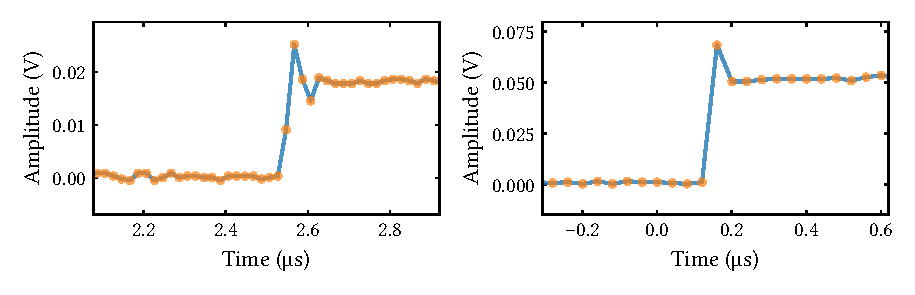
\includegraphics{figures/eom_rise_155.pdf}
	\caption{The efficiency of the \acp{eom} were evaluated by setting the polarization of the incoming light either horizontal or vertical using the waveplate. The pockels cell will then periodically turn the polarization $\SI{90}{\degree}$, which can be seen by measuring the voltage on the photodiode.}
}
\end{figure}

Moving on from the rise times, it is important to measure how much light is left when the light is supposed to be off, after filtering it from the \ac{pbs}. The measure in question is the extinction ratio and is evaluated by the ratio of the $high$ to the $low$ level of the signal. Figure~\ref{fig:eom_extinction} shows signals taken for both crystals using the same setup as before. In order to correctly evaluate both levels, it is necessary to note that photodiodes are susceptible to dark noise, which is electrical noise falsely registered as light. This means a dark image was taken, with the laser beam off, and the mean of the dark image was subtracted from the signals used to evaluate the extinction ratio. The high and low levels are then found by selecting points of the respective level after it has stabilized, the ranges for which are given in Figure~\ref{fig:eom_extinction}.
Not considering the standard deviation on the dark level, already the standard deviation on the low level for both crystals is on the order of the mean, which makes it impossible to give an upper bound to the extinction ratio, the values for both are summarized in the following table.

\begin{center}
\begin{tabular}{l|l|l|l|l|l}
	\hline \hline
	& $upper$ & $\sigma_{upper}$ & $lower$ & $\sigma_{lower}$ & $upper/lower$ \\
	\thickhline
	RTP & \num{1.9e-02} & \num{6.2e-04} & \num{3.7e-04} & \num{5.2e-04} & \num{5.1e+01} \\
	BBO & \num{1.9e-02} & \num{8.3e-04} & \num{9.6e-04} & \num{7.4e-04} & \num{5.7e+01} \\
	\hline \hline
\end{tabular}
\end{center}

However, the lower bound is the mean of the level, which for \ac{rtp} gives $51:1$ and for \ac{bbo} gives $57:1$. The manufacturer provides an extinction ratio for the \ac{rtp} crystal of $> 200:1$, however no value is given for \ac{bbo}. This means, that our measurement is limited by the photodiode and in order to validate the value given by the manufacturer, it is necessary to reduce the dark noise for example by cooling the diode.

\begin{figure}[t]
\label{fig:eom_extinction}
\centering{%
	\setlength{\figureheight}{2in}
	\setlength{\figurewidth}{\textwidth/2-2.5em}
	%% This file was created by tikzplotlib v0.9.4.
\begin{tikzpicture}

\definecolor{color0}{rgb}{0.12156862745098,0.466666666666667,0.705882352941177}
\definecolor{color1}{rgb}{1,0.498039215686275,0.0549019607843137}

\begin{groupplot}[group style={group size=2 by 1, horizontal sep=5em}]
\nextgroupplot[
height=\figureheight,
minor xtick={},
minor ytick={},
scaled y ticks=false,
tick align=inside,
tick pos=both,
width=\figurewidth,
x grid style={white!69.0196078431373!black},
xlabel={Time (ms)},
xmin=-5.00806, xmax=5.88194,
xtick style={color=black},
xtick={-6,-4,-2,0,2,4,6},
y grid style={white!69.0196078431373!black},
y tick label style={/pgf/number format/fixed},
ylabel style={align=center},
ylabel={Amplitude (a. u.)},
ymin=-0.00684806308564516, ymax=0.0267013484143548,
ytick style={color=black},
ytick={-0.01,-0.005,0,0.005,0.01,0.015,0.02,0.025,0.03}
]
\addplot [line width=1.5pt, color0]
table {%
-4.51306 0.0191854151643548
-4.49306 0.0197300451643548
-4.47306 0.0186407751643548
-4.45306 0.0189130951643548
-4.43306 0.0189130951643548
-4.41306 0.0191854151643548
-4.39306 0.0191854151643548
-4.37306 0.0186407751643548
-4.35306 0.0194577251643548
-4.33306 0.0183684651643548
-4.31306 0.0191854151643548
-4.29306 0.0189130951643548
-4.27306 0.0194577251643548
-4.25306 0.0189130951643548
-4.23306 0.0191854151643548
-4.21306 0.0194577251643548
-4.19306 0.0194577251643548
-4.17306 0.0194577251643548
-4.15306 0.0186407751643548
-4.13306 0.0186407751643548
-4.11306 0.0194577251643548
-4.09306 0.0189130951643548
-4.07306 0.0189130951643548
-4.05306 0.0189130951643548
-4.03306 0.0183684651643548
-4.01306 0.0189130951643548
-3.99306 0.0189130951643548
-3.97306 0.0183684651643548
-3.95306 0.0183684651643548
-3.93306 0.0186407751643548
-3.91306 0.0191854151643548
-3.89306 0.0191854151643548
-3.87306 0.0186407751643548
-3.85306 0.0194577251643548
-3.83306 0.0191854151643548
-3.81306 0.0186407751643548
-3.79306 0.0186407751643548
-3.77306 0.0191854151643548
-3.75306 0.0186407751643548
-3.73306 0.0191854151643548
-3.71306 0.0197300451643548
-3.69306 0.0189130951643548
-3.67306 0.0191854151643548
-3.65306 0.0194577251643548
-3.63306 0.0186407751643548
-3.61306 0.0186407751643548
-3.59306 0.0183684651643548
-3.57306 0.0197300451643548
-3.55306 0.0186407751643548
-3.53306 0.0191854151643548
-3.51306 0.0191854151643548
-3.49306 0.0186407751643548
-3.47306 0.0205469951643548
-3.45306 0.0167345651643548
-3.43306 0.0191854151643548
-3.41306 0.0200023651643548
-3.39306 0.0202746751643548
-3.37306 0.0183684651643548
-3.35306 0.0178238251643548
-3.33306 0.0208193151643548
-3.31306 0.0172791951643548
-3.29306 0.0183684651643548
-3.27306 0.0183684651643548
-3.25306 0.0205469951643548
-3.23306 0.0197300451643548
-3.21306 0.0183684651643548
-3.19306 0.0178238251643548
-3.17306 0.0178238251643548
-3.15306 0.0200023651643548
-3.13306 0.0191854151643548
-3.11306 0.0202746751643548
-3.09306 0.0178238251643548
-3.07306 0.0189130951643548
-3.05306 0.0191854151643548
-3.03306 0.0189130951643548
-3.01306 0.0200023651643548
-2.99306 0.0183684651643548
-2.97306 0.0186407751643548
-2.95306 0.0189130951643548
-2.93306 0.0200023651643548
-2.91306 0.0183684651643548
-2.89306 0.0194577251643548
-2.87306 0.0191854151643548
-2.85306 0.0202746751643548
-2.83306 0.0183684651643548
-2.81306 0.0191854151643548
-2.79306 0.0189130951643548
-2.77306 0.0186407751643548
-2.75306 0.0197300451643548
-2.73306 0.0186407751643548
-2.71306 0.0186407751643548
-2.69306 0.0183684651643548
-2.67306 0.0183684651643548
-2.65306 0.0194577251643548
-2.63306 0.0189130951643548
-2.61306 0.0200023651643548
-2.59306 0.0183684651643548
-2.57306 0.0194577251643548
-2.55306 0.0189130951643548
-2.53306 0.0189130951643548
-2.51306 0.0183684651643548
-2.49306 0.0205469951643548
-2.47306 0.0178238251643548
-2.45306 0.00475262816435484
-2.43306 -0.00532308983564516
-2.41306 0.00148482716435484
-2.39306 0.00121251116435484
-2.37306 -0.000421389335645161
-2.35306 0.000940194164354839
-2.33306 0.000940194164354839
-2.31306 0.00175714416435484
-2.29306 0.000667877164354839
-2.27306 0.000123244064354839
-2.25306 0.000940194164354839
-2.23306 0.000667877164354839
-2.21306 0.00121251116435484
-2.19306 0.000395561164354839
-2.17306 0.000395561164354839
-2.15306 0.00175714416435484
-2.13306 0.000940194164354839
-2.11306 -0.000421389335645161
-2.09306 0.000395561164354839
-2.07306 0.000667877164354839
-2.05306 0.00148482716435484
-2.03306 -0.000149072635645161
-2.01306 0.00202946116435484
-1.99306 0.000940194164354839
-1.97306 0.000395561164354839
-1.95306 0.000395561164354839
-1.93306 0.000123244064354839
-1.91306 0.000123244064354839
-1.89306 0.000395561164354839
-1.87306 0.000940194164354839
-1.85306 0.00121251116435484
-1.83306 0.000667877164354839
-1.81306 0.000940194164354839
-1.79306 0.000395561164354839
-1.77306 0.00121251116435484
-1.75306 0.000123244064354839
-1.73306 0.00121251116435484
-1.71306 0.000667877164354839
-1.69306 -0.000421389335645161
-1.67306 0.000395561164354839
-1.65306 0.000667877164354839
-1.63306 0.000395561164354839
-1.61306 -0.000421389335645161
-1.59306 0.000940194164354839
-1.57306 0.000940194164354839
-1.55306 0.000123244064354839
-1.53306 0.000940194164354839
-1.51306 0.000395561164354839
-1.49306 0.000940194164354839
-1.47306 0.000123244064354839
-1.45306 0.000123244064354839
-1.43306 0.000123244064354839
-1.41306 -0.000149072635645161
-1.39306 0.000667877164354839
-1.37306 0.000940194164354839
-1.35306 -0.000149072635645161
-1.33306 0.000395561164354839
-1.31306 0.00121251116435484
-1.29306 -0.000149072635645161
-1.27306 0.000667877164354839
-1.25306 0.000395561164354839
-1.23306 0.000123244064354839
-1.21306 0.000940194164354839
-1.19306 0.000395561164354839
-1.17306 0.000940194164354839
-1.15306 -0.000149072635645161
-1.13306 0.000940194164354839
-1.11306 0.000940194164354839
-1.09306 0.000940194164354839
-1.07306 0.000123244064354839
-1.05306 0.000395561164354839
-1.03306 0.000940194164354839
-1.01306 -0.000149072635645161
-0.993064 0.000667877164354839
-0.973064 0.000940194164354839
-0.953064 0.000395561164354839
-0.933064 -0.000149072635645161
-0.913064 0.000940194164354839
-0.893064 -0.000421389335645161
-0.873064 0.000940194164354839
-0.853064 0.000940194164354839
-0.833064 0.000395561164354839
-0.813064 0.000395561164354839
-0.793064 0.000667877164354839
-0.773064 0.000940194164354839
-0.753064 -0.000421389335645161
-0.733064 0.000667877164354839
-0.713064 0.000940194164354839
-0.693064 -0.000149072635645161
-0.673064 0.000667877164354839
-0.653064 0.000395561164354839
-0.633064 -0.000149072635645161
-0.613064 -0.000149072635645161
-0.593064 0.000667877164354839
-0.573064 -0.000421389335645161
-0.553064 0.000123244064354839
-0.533064 0.000395561164354839
-0.513064 -0.000149072635645161
-0.493064 0.000123244064354839
-0.473064 0.000940194164354839
-0.453064 0.000395561164354839
-0.433064 -0.000149072635645161
-0.413064 0.000940194164354839
-0.393064 0.000667877164354839
-0.373064 0.000123244064354839
-0.353064 0.000667877164354839
-0.333064 0.00121251116435484
-0.313064 0.000123244064354839
-0.293064 -0.000149072635645161
-0.273064 0.000667877164354839
-0.253064 0.000940194164354839
-0.233064 0.000395561164354839
-0.213064 -0.000149072635645161
-0.193064 -0.000421389335645161
-0.173064 0.000940194164354839
-0.153064 0.000395561164354839
-0.133064 0.000395561164354839
-0.113064 0.000123244064354839
-0.0930644 0.000395561164354839
-0.0730644 0.000395561164354839
-0.0530644 0.000123244064354839
-0.0330644 -0.000693706035645161
-0.0130644 0.000395561164354839
0.00693559 0.000940194164354839
0.0269356 0.000667877164354839
0.0469356 0.000395561164354839
0.0669356 -0.00123833933564516
0.0869356 0.000940194164354839
0.106936 -0.000149072635645161
0.126936 0.000395561164354839
0.146936 -0.000149072635645161
0.166936 0.000395561164354839
0.186936 0.000395561164354839
0.206936 0.000395561164354839
0.226936 0.000940194164354839
0.246936 0.000940194164354839
0.266936 -0.000149072635645161
0.286936 0.000123244064354839
0.306936 0.000395561164354839
0.326936 0.000940194164354839
0.346936 0.000667877164354839
0.366936 0.000940194164354839
0.386936 0.000123244064354839
0.406936 -0.000693706035645161
0.426936 0.000940194164354839
0.446936 0.000395561164354839
0.466936 0.000940194164354839
0.486936 0.000123244064354839
0.506936 0.000667877164354839
0.526936 0.000940194164354839
0.546936 -0.000149072635645161
0.566936 0.000395561164354839
0.586936 0.000940194164354839
0.606936 0.000395561164354839
0.626936 0.000123244064354839
0.646936 0.000395561164354839
0.666936 0.000395561164354839
0.686936 0.000395561164354839
0.706936 -0.000149072635645161
0.726936 0.000667877164354839
0.746936 -0.000149072635645161
0.766936 0.000123244064354839
0.786936 0.000395561164354839
0.806936 0.000123244064354839
0.826936 0.000667877164354839
0.846936 -0.000421389335645161
0.866936 0.000667877164354839
0.886936 0.000123244064354839
0.906936 -0.000149072635645161
0.926936 0.000940194164354839
0.946936 0.000395561164354839
0.966936 0.000395561164354839
0.986936 0.000123244064354839
1.00694 0.000940194164354839
1.02694 0.000395561164354839
1.04694 0.000123244064354839
1.06694 0.000395561164354839
1.08694 0.000395561164354839
1.10694 0.000395561164354839
1.12694 -0.000149072635645161
1.14694 0.000667877164354839
1.16694 0.000940194164354839
1.18694 -0.000149072635645161
1.20694 0.000395561164354839
1.22694 -0.000149072635645161
1.24694 0.000123244064354839
1.26694 0.000395561164354839
1.28694 0.000395561164354839
1.30694 0.000395561164354839
1.32694 0.000395561164354839
1.34694 0.000123244064354839
1.36694 0.000123244064354839
1.38694 0.00121251116435484
1.40694 -0.000693706035645161
1.42694 0.000667877164354839
1.44694 -0.000421389335645161
1.46694 0.000123244064354839
1.48694 -0.000421389335645161
1.50694 -0.000693706035645161
1.52694 0.000940194164354839
1.54694 -0.000149072635645161
1.56694 0.000667877164354839
1.58694 0.000123244064354839
1.60694 0.000123244064354839
1.62694 -0.000421389335645161
1.64694 0.000395561164354839
1.66694 0.000123244064354839
1.68694 -0.000149072635645161
1.70694 0.000940194164354839
1.72694 -0.000149072635645161
1.74694 0.000940194164354839
1.76694 0.000395561164354839
1.78694 -0.00123833933564516
1.80694 -0.000149072635645161
1.82694 0.000940194164354839
1.84694 0.000395561164354839
1.86694 0.00202946116435484
1.88694 0.000667877164354839
1.90694 0.000123244064354839
1.92694 -0.000966022735645161
1.94694 -0.000421389335645161
1.96694 0.00121251116435484
1.98694 -0.000149072635645161
2.00694 0.000667877164354839
2.02694 0.000395561164354839
2.04694 -0.000421389335645161
2.06694 0.000667877164354839
2.08694 0.000940194164354839
2.10694 0.000940194164354839
2.12694 0.000395561164354839
2.14694 -0.000149072635645161
2.16694 -0.000421389335645161
2.18694 0.000940194164354839
2.20694 0.000940194164354839
2.22694 -0.000421389335645161
2.24694 0.000123244064354839
2.26694 0.000940194164354839
2.28694 0.000123244064354839
2.30694 0.000395561164354839
2.32694 0.000395561164354839
2.34694 0.000123244064354839
2.36694 0.000123244064354839
2.38694 -0.000421389335645161
2.40694 0.000395561164354839
2.42694 0.000395561164354839
2.44694 0.000395561164354839
2.46694 0.000395561164354839
2.48694 -0.000149072635645161
2.50694 0.000123244064354839
2.52694 0.000395561164354839
2.54694 0.00910969416435484
2.56694 0.0251763751643548
2.58694 0.0186407751643548
2.60694 0.0145560251643548
2.62694 0.0189130951643548
2.64694 0.0183684651643548
2.66694 0.0178238251643548
2.68694 0.0178238251643548
2.70694 0.0178238251643548
2.72694 0.0183684651643548
2.74694 0.0178238251643548
2.76694 0.0178238251643548
2.78694 0.0183684651643548
2.80694 0.0186407751643548
2.82694 0.0186407751643548
2.84694 0.0183684651643548
2.86694 0.0178238251643548
2.88694 0.0186407751643548
2.90694 0.0183684651643548
2.92694 0.0178238251643548
2.94694 0.0186407751643548
2.96694 0.0183684651643548
2.98694 0.0186407751643548
3.00694 0.0189130951643548
3.02694 0.0186407751643548
3.04694 0.0175515151643548
3.06694 0.0186407751643548
3.08694 0.0186407751643548
3.10694 0.0180961451643548
3.12694 0.0183684651643548
3.14694 0.0194577251643548
3.16694 0.0183684651643548
3.18694 0.0191854151643548
3.20694 0.0189130951643548
3.22694 0.0186407751643548
3.24694 0.0189130951643548
3.26694 0.0186407751643548
3.28694 0.0191854151643548
3.30694 0.0180961451643548
3.32694 0.0189130951643548
3.34694 0.0189130951643548
3.36694 0.0189130951643548
3.38694 0.0200023651643548
3.40694 0.0183684651643548
3.42694 0.0186407751643548
3.44694 0.0186407751643548
3.46694 0.0189130951643548
3.48694 0.0186407751643548
3.50694 0.0191854151643548
3.52694 0.0186407751643548
3.54694 0.0194577251643548
3.56694 0.0194577251643548
3.58694 0.0191854151643548
3.60694 0.0191854151643548
3.62694 0.0189130951643548
3.64694 0.0197300451643548
3.66694 0.0183684651643548
3.68694 0.0191854151643548
3.70694 0.0191854151643548
3.72694 0.0186407751643548
3.74694 0.0191854151643548
3.76694 0.0191854151643548
3.78694 0.0186407751643548
3.80694 0.0194577251643548
3.82694 0.0191854151643548
3.84694 0.0186407751643548
3.86694 0.0183684651643548
3.88694 0.0194577251643548
3.90694 0.0197300451643548
3.92694 0.0197300451643548
3.94694 0.0183684651643548
3.96694 0.0183684651643548
3.98694 0.0202746751643548
4.00694 0.0186407751643548
4.02694 0.0189130951643548
4.04694 0.0189130951643548
4.06694 0.0200023651643548
4.08694 0.0178238251643548
4.10694 0.0194577251643548
4.12694 0.0175515151643548
4.14694 0.0197300451643548
4.16694 0.0191854151643548
4.18694 0.0194577251643548
4.20694 0.0191854151643548
4.22694 0.0197300451643548
4.24694 0.0189130951643548
4.26694 0.0194577251643548
4.28694 0.0191854151643548
4.30694 0.0189130951643548
4.32694 0.0189130951643548
4.34694 0.0186407751643548
4.36694 0.0191854151643548
4.38694 0.0183684651643548
4.40694 0.0189130951643548
4.42694 0.0197300451643548
4.44694 0.0191854151643548
4.46694 0.0200023651643548
4.48694 0.0189130951643548
4.50694 0.0194577251643548
4.52694 0.0183684651643548
4.54694 0.0191854151643548
4.56694 0.0197300451643548
4.58694 0.0183684651643548
4.60694 0.0183684651643548
4.62694 0.0200023651643548
4.64694 0.0183684651643548
4.66694 0.0183684651643548
4.68694 0.0186407751643548
4.70694 0.0189130951643548
4.72694 0.0186407751643548
4.74694 0.0194577251643548
4.76694 0.0189130951643548
4.78694 0.0194577251643548
4.80694 0.0183684651643548
4.82694 0.0194577251643548
4.84694 0.0191854151643548
4.86694 0.0186407751643548
4.88694 0.0175515151643548
4.90694 0.0189130951643548
4.92694 0.0191854151643548
4.94694 0.0191854151643548
4.96694 0.0183684651643548
4.98694 0.0194577251643548
5.00694 0.0191854151643548
5.02694 0.0191854151643548
5.04694 0.0191854151643548
5.06694 0.0189130951643548
5.08694 0.0194577251643548
5.10694 0.0191854151643548
5.12694 0.0191854151643548
5.14694 0.0186407751643548
5.16694 0.0197300451643548
5.18694 0.0186407751643548
5.20694 0.0186407751643548
5.22694 0.0197300451643548
5.24694 0.0189130951643548
5.26694 0.0194577251643548
5.28694 0.0183684651643548
5.30694 0.0194577251643548
5.32694 0.0194577251643548
5.34694 0.0197300451643548
5.36694 0.0186407751643548
5.38694 0.0197300451643548
};
\addplot [line width=1.5pt, color1, dashed]
table {%
-4.51306 0.0192932717552554
-4.49306 0.0193105152472244
-4.47306 0.0193194754466001
-4.45306 0.0193198861860666
-4.43306 0.019311702759259
-4.41306 0.0192951029399212
-4.39306 0.0192704826600563
-4.37306 0.0192384464450048
-4.35306 0.0191997928217822
-4.33306 0.019155495030766
-4.31306 0.0191066774775032
-4.29306 0.0190545884586945
-4.27306 0.0190005697822049
-4.25306 0.01894602397337
-4.23306 0.0188923798173238
-4.21306 0.018841057028294
-4.19306 0.0187934308608322
-4.17306 0.0187507974842101
-4.15306 0.0187143409294841
-4.13306 0.0186851023891957
-4.11306 0.0186639526028562
-4.09306 0.0186515679981872
-4.07306 0.0186484111797911
-4.05306 0.0186547162650967
-4.03306 0.0186704794639303
-4.01306 0.0186954551850257
-3.99306 0.0187291578325461
-3.97306 0.0187708693307452
-3.95306 0.0188196522878604
-3.93306 0.0188743685838846
-3.91306 0.018933703043684
-3.89306 0.0189961917396485
-3.87306 0.0190602543592202
-3.85306 0.0191242299745972
-3.83306 0.0191864154668433
-3.81306 0.0192451057864565
-3.79306 0.0192986351787853
-3.77306 0.0193454184668364
-3.75306 0.0193839914669325
-3.73306 0.0194130496149158
-3.71306 0.0194314839023381
-3.69306 0.019438413263095
-3.67306 0.0194332126106451
-3.65306 0.0194155358032932
-3.63306 0.0193853329086328
-3.61306 0.0193428612464274
-3.59306 0.0192886898099227
-3.57306 0.0192236967965274
-3.55306 0.0191490601174309
-3.53306 0.0190662408993417
-3.51306 0.0189769601372754
-3.49306 0.0188831688022828
-3.47306 0.0187870118492568
-3.45306 0.0186907867046052
-3.43306 0.0185968969388332
-3.41306 0.0185078019423205
-3.39306 0.0184259635213819
-3.37306 0.0183537904139117
-3.35306 0.0182935817876725
-3.33306 0.0182474708280952
-3.31306 0.0182173695451749
-3.29306 0.01820491592994
-3.27306 0.0182114245697467
-3.25306 0.0182378417883999
-3.23306 0.0182847063124079
-3.21306 0.0183521163794801
-3.19306 0.0184397041010908
-3.17306 0.0185466177692926
-3.15306 0.0186715126611159
-3.13306 0.0188125507442539
-3.11306 0.0189674095280195
-3.09306 0.0191333001366991
-3.07306 0.0193069945115044
-3.05306 0.0194848614755435
-3.03306 0.0196629112268434
-3.01306 0.0198368476606854
-2.99306 0.0200021277675251
-2.97306 0.0201540272095697
-2.95306 0.0202877110505091
-2.93306 0.0203983085014979
-2.91306 0.0204809904545475
-2.89306 0.0205310485039156
-2.87306 0.0205439741084153
-2.85306 0.0205155365239227
-2.83306 0.0204418581364072
-2.81306 0.0203194858517665
-2.79306 0.0201454572493635
-2.77306 0.0199173602807247
-2.75306 0.0196333853922115
-2.73306 0.0192923690690123
-2.71306 0.0188938279355346
-2.69306 0.0184379827018248
-2.67306 0.0179257714143185
-2.65306 0.0173588516490463
-2.63306 0.0167395914731999
-2.61306 0.0160710491933257
-2.59306 0.015356942101907
-2.57306 0.0146016046252101
-2.55306 0.0138099364605241
-2.53306 0.0129873414669471
-2.51306 0.0121396582374213
-2.49306 0.0112730834277867
-2.47306 0.010394089048474
-2.45306 0.00950933503366322
-2.43306 0.00862557848926327
-2.41306 0.0077495810832746
-2.39306 0.00688801607878963
-2.37306 0.006047376520338
-2.35306 0.00523388606823347
-2.33306 0.00445341393326998
-2.31306 0.00371139529625196
-2.29306 0.00301275850461105
-2.27306 0.00236186022338972
-2.25306 0.00176242958220268
-2.23306 0.00121752220585071
-2.21306 0.000729484846814451
-2.19306 0.00029993115594793
-2.17306 -7.02710634075936e-05
-2.15306 -0.000381000969516354
-2.13306 -0.000632874215226602
-2.11306 -0.000827221148189602
-2.09306 -0.000966054119418242
-2.07306 -0.00105202452563901
-2.05306 -0.0010883703835544
-2.03306 -0.0010788553920246
-2.01306 -0.00102770057849116
-1.99306 -0.00093950974622543
-1.97306 -0.000819190037086826
-1.95306 -0.000671868998728946
-1.93306 -0.000502809594346653
-1.91306 -0.000317324616329717
-1.89306 -0.000120691962273635
-1.87306 8.19277971274499e-05
-1.85306 0.000285570183061291
-1.83306 0.000485540609721431
-1.81306 0.000677482026029462
-1.79306 0.000857435324290915
-1.77306 0.00102189158234564
-1.75306 0.00116783536166645
-1.73306 0.00129277845246367
-1.71306 0.00139478363499051
-1.69306 0.00147247821057697
-1.67306 0.00152505724301159
-1.65306 0.00155227663727145
-1.63306 0.00155443636483512
-1.61306 0.00153235431955976
-1.59306 0.00148733145218174
-1.57306 0.00142110898194713
-1.55306 0.00133581861800422
-1.53306 0.00123392683862872
-1.51306 0.00111817437110071
-1.49306 0.000991512087513277
-1.47306 0.000857034580794072
-1.45306 0.000717912710046141
-1.43306 0.000577326404702719
-1.41306 0.000438398993149205
-1.39306 0.000304134274057588
-1.37306 0.000177357478808758
-1.35306 6.06611825714788e-05
-1.33306 -4.36428882244315e-05
-1.31306 -0.000133565330879201
-1.29306 -0.000207473143531886
-1.27306 -0.000264115876217804
-1.25306 -0.000302643488249821
-1.23306 -0.000322615710056817
-1.21306 -0.000324002875353693
-1.19306 -0.000307178355995686
-1.17306 -0.00027290289388875
-1.15306 -0.00022230127879864
-1.13306 -0.000156831964904782
-1.11306 -7.82503497844065e-05
-1.09306 1.1433445233619e-05
-1.07306 0.000110001356839348
-1.05306 0.00021507770899497
-1.03306 0.000324182017676708
-1.01306 0.000434783163480877
-0.993064 0.000544332166065919
-0.973064 0.000650403258946407
-0.953064 0.000750613263206291
-0.933064 0.000842758668899668
-0.913064 0.000924838233475255
-0.893064 0.000995092880769875
-0.873064 0.00105204003925455
-0.853064 0.00109450177991163
-0.833064 0.0011216262466384
-0.813064 0.00113290201352862
-0.793064 0.00112816515089649
-0.773064 0.00110759893249333
-0.753064 0.0010717262670005
-0.733064 0.00102139508455416
-0.713064 0.00095775705083838
-0.693064 0.000882240114375793
-0.673064 0.000796515514444041
-0.653064 0.000702459985183613
-0.633064 0.000602113983858408
-0.613064 0.00049763684612928
-0.593064 0.000391259827205869
-0.573064 0.000285238023843766
-0.553064 0.000181802187743801
-0.533064 8.31114357950757e-05
-0.513064 -8.79216299380821e-06
-0.493064 -9.20261894787021e-05
-0.473064 -0.000164906795151765
-0.453064 -0.000225983153264338
-0.433064 -0.000274066749229267
-0.413064 -0.00030825493021819
-0.393064 -0.000327948256158873
-0.373064 -0.000332861325392493
-0.353064 -0.000323026885365774
-0.333064 -0.000298793179092859
-0.313064 -0.000260814618853548
-0.293064 -0.000210036016830418
-0.273064 -0.000147670735317114
-0.253064 -7.51732440617582e-05
-0.233064 5.79331327977411e-06
-0.213064 9.3393840018061e-05
-0.193064 0.000185661504340557
-0.173064 0.000280540593825793
-0.153064 0.000375931093965805
-0.133064 0.000469734044934831
-0.113064 0.000559896717307199
-0.0930644 0.000644455031045084
-0.0730644 0.000721582192954207
-0.0530644 0.000789617531963582
-0.0330644 0.000847108697404784
-0.0130644 0.000892840682615096
0.00693559 0.000925861446270299
0.0269356 0.000945501935811443
0.0469356 0.000951389820526611
0.0669356 0.000943457109511566
0.0869356 0.000921941038938914
0.106936 0.000887377673018551
0.126936 0.000840592912852212
0.146936 0.000782680127989067
0.166936 0.000714978692770273
0.186936 0.000639044159361673
0.206936 0.000556614330753605
0.226936 0.000469571386553066
0.246936 0.000379900861001505
0.266936 0.000289648339698228
0.286936 0.000200874790667988
0.306936 0.000115611475646968
0.326936 3.58153981275446e-05
0.346936 -3.66737644551616e-05
0.366936 -0.000100174325838736
0.386936 -0.000153199982740248
0.406936 -0.000194493128864499
0.426936 -0.00022305336960652
0.446936 -0.000238160614125151
0.466936 -0.000239392232877483
0.486936 -0.000226633891098855
0.506936 -0.000200083799614444
0.526936 -0.000160250261120928
0.546936 -0.000107942529897974
0.566936 -4.42551429472651e-05
0.586936 2.94539820554253e-05
0.606936 0.000111591254693635
0.626936 0.000200360374604917
0.646936 0.000293799885147645
0.666936 0.000389824554100844
0.686936 0.000486269732922907
0.706936 0.000580937778476776
0.726936 0.000671645571991522
0.746936 0.000756272140472166
0.766936 0.000832805376496395
0.786936 0.000899386863651142
0.806936 0.000954353846650353
0.826936 0.000996277436911543
0.846936 0.0010239962151232
0.866936 0.00103664448078979
0.886936 0.00103367450321573
0.906936 0.00101487224687229
0.926936 0.000980366174279549
0.946936 0.000930628868877073
0.966936 0.000866471366102994
0.986936 0.000789030230158417
1.00694 0.000699728633223696
1.02694 0.000600323519694849
1.04694 0.000492764964810623
1.06694 0.000379226973059697
1.08694 0.000262047213026617
1.10694 0.000143679405314786
1.12694 2.66425720585016e-05
1.14694 -8.65318429362997e-05
1.16694 -0.000193353918921427
1.18694 -0.000291429168641284
1.20694 -0.000378511302306289
1.22694 -0.000452552742039068
1.24694 -0.000511751814940502
1.26694 -0.00055459560582149
1.28694 -0.000579897524374984
1.30694 -0.000586828734850824
1.32694 -0.000574942707479468
1.34694 -0.00054419227794497
1.36694 -0.000494938741781281
1.38694 -0.000427952662028703
1.40694 -0.000344406227976797
1.42694 -0.000245857167296321
1.44694 -0.000134224380169856
1.46694 -1.17556289505397e-05
1.48694 0.000119012222798752
1.50694 0.000255299775455244
1.52694 0.000394137674428533
1.54694 0.0005324242907267
1.56694 0.000666987472490874
1.58694 0.000794649245437464
1.60694 0.000912292267030574
1.62694 0.00101692678810997
1.64694 0.00110575684778871
1.66694 0.00117624442344392
1.68694 0.00122617027783398
1.70694 0.00125369028960781
1.72694 0.0012573861210901
1.74694 0.0012363091671447
1.76694 0.00119001683962115
1.78694 0.00111860037145857
1.80694 0.00102270347066799
1.82694 0.000903531314525221
1.84694 0.0007628495454874
1.86694 0.00060297310947947
1.88694 0.00042674496099503
1.90694 0.000237504844529684
1.92694 3.9048544778637e-05
1.94694 -0.000164421824625305
1.96694 -0.00036835575560667
1.98694 -0.000567919608765333
2.00694 -0.000758068169154951
2.02694 -0.000933621335134131
2.04694 -0.00108934467718246
2.06694 -0.00122003252217319
2.08694 -0.00132059216092498
2.10694 -0.00138612774409286
2.12694 -0.00141202242432397
2.14694 -0.00139401732134274
2.16694 -0.00132828593101322
2.18694 -0.0012115026687464
2.20694 -0.00104090433071137
2.22694 -0.000814343371559289
2.24694 -0.000530332032757768
2.26694 -0.000188076508762135
2.28694 0.000212499493609443
2.30694 0.000670742267087542
2.32694 0.00118526696273029
2.34694 0.00175396787687313
2.36694 0.00237404005141034
2.38694 0.0030420118781008
2.40694 0.00375378820830509
2.42694 0.00450470328887641
2.44694 0.00528958267610332
2.46694 0.00610281312567575
2.48694 0.00693841932039011
2.50694 0.00779014618115893
2.52694 0.00865154541292341
2.54694 0.0095160648669403
2.56694 0.0103771392558563
2.58694 0.0112282807387526
2.60694 0.0120631679002309
2.62694 0.0128757316804279
2.64694 0.0136602368709233
2.66694 0.0144113578737224
2.68694 0.0151242475252818
2.70694 0.0157945979129338
2.72694 0.016418692254701
2.74694 0.0169934470727222
2.76694 0.0175164440623598
2.78694 0.0179859512403944
2.80694 0.0184009331431735
2.82694 0.0187610500357721
2.84694 0.0190666462826634
2.86694 0.0193187282156758
2.88694 0.019518932012781
2.90694 0.0196694822683607
2.92694 0.0197731420890497
2.94694 0.0198331556863873
2.96694 0.0198531845559324
2.98694 0.0198372384302093
3.00694 0.0197896022682408
3.02694 0.0197147605962883
3.04694 0.0196173205420327
3.06694 0.0195019349074871
3.08694 0.0193732266046217
3.10694 0.0192357157326171
3.12694 0.0190937505079159
3.14694 0.0189514431692875
3.16694 0.0188126118718338
3.18694 0.0186807294584415
3.20694 0.0185588798571613
3.22694 0.0184497227011247
3.24694 0.018355466606868
3.26694 0.0182778513804287
3.28694 0.0182181392515055
3.30694 0.0181771150675321
3.32694 0.0181550952148867
3.34694 0.0181519448766974
3.36694 0.0181671030887233
3.38694 0.0181996149192816
3.40694 0.0182481699785712
3.42694 0.0183111463591488
3.44694 0.0183866590244881
3.46694 0.0184726115979139
3.48694 0.018566750460719
3.50694 0.0186667200465195
3.52694 0.0187701182190262
3.54694 0.0188745506421214
3.56694 0.0189776830937284
3.58694 0.0190772907373531
3.60694 0.0191713034458753
3.62694 0.0192578463693672
3.64694 0.0193352750502829
3.66694 0.0194022045129163
3.68694 0.0194575318869708
3.70694 0.0195004522646594
3.72694 0.0195304676341139
3.74694 0.0195473888761023
3.76694 0.0195513309532622
3.78694 0.0195427015584121
3.80694 0.019522183618314
3.82694 0.0194907121690039
3.84694 0.0194494462261804
3.86694 0.0193997363671262
3.88694 0.0193430888175079
3.90694 0.0192811268957868
3.92694 0.0192155507088552
3.94694 0.019148096014272
3.96694 0.0190804931668649
3.98694 0.0190144270506628
4.00694 0.0189514988616597
4.02694 0.0188931905537349
4.04694 0.0188408326904211
4.06694 0.0187955763607517
4.08694 0.0187583697200132
4.10694 0.0187299396080372
4.12694 0.0187107785810417
4.14694 0.0187011375704917
4.16694 0.0187010242566024
4.18694 0.0187102071176377
4.20694 0.0187282249917155
4.22694 0.0187544018680332
4.24694 0.0187878665117661
4.26694 0.0188275764236952
4.28694 0.0188723455440238
4.30694 0.0189208750317023
4.32694 0.0189717863874891
4.34694 0.0190236561421874
4.36694 0.0190750513019251
4.38694 0.019124564730544
4.40694 0.0191708496553026
4.42694 0.0192126525059766
4.44694 0.0192488433384914
4.46694 0.0192784431515024
4.48694 0.0193006474765856
4.50694 0.0193148457083313
4.52694 0.0193206357377735
4.54694 0.0193178335591503
4.56694 0.0193064776336637
4.58694 0.0192868279122526
4.60694 0.0192593595398611
4.62694 0.0192247513836881
4.64694 0.0191838696448659
4.66694 0.0191377469244122
4.68694 0.0190875572177355
4.70694 0.0190345874052095
4.72694 0.018980205887335
4.74694 0.0189258290800235
4.76694 0.0188728865370601
4.78694 0.0188227855017056
4.80694 0.0187768757068369
4.82694 0.0187364152425854
4.84694 0.0187025382920191
4.86694 0.0186762254993478
4.88694 0.0186582776820867
4.90694 0.0186492935296277
4.92694 0.0186496518471235
4.94694 0.0186594988071749
4.96694 0.0186787405644965
4.98694 0.0187070414727268
5.00694 0.018743828020256
5.02694 0.0187882984759075
5.04694 0.0188394381081811
5.06694 0.0188960397162237
5.08694 0.0189567290894156
5.10694 0.0190199948980346
5.12694 0.0190842224123817
5.14694 0.0191477303543034
5.16694 0.0192088101053256
5.18694 0.0192657664314237
5.20694 0.0193169588373009
5.22694 0.0193608426341156
5.24694 0.0193960087946693
5.26694 0.0194212216795883
5.28694 0.0194354537470108
5.30694 0.0194379164063667
5.32694 0.0194280862432434
5.34694 0.0194057259259242
5.36694 0.0193708992034513
5.38694 0.0193239795181823
};

\nextgroupplot[
height=\figureheight,
minor xtick={},
minor ytick={},
scaled y ticks=false,
tick align=inside,
tick pos=both,
width=\figurewidth,
x grid style={white!69.0196078431373!black},
xlabel={Time (ms)},
xmin=-10.4293315, xmax=11.3507015,
xtick style={color=black},
xtick={-15,-10,-5,0,5,10,15},
y grid style={white!69.0196078431373!black},
y tick label style={/pgf/number format/fixed},
ylabel style={align=center},
ylabel={Amplitude (a. u.)},
ymin=-0.0147315379356452, ymax=0.0722397662643548,
ytick style={color=black},
ytick={-0.02,-0.01,0,0.01,0.02,0.03,0.04,0.05,0.06,0.07,0.08}
]
\addplot [line width=1.5pt, color0]
table {%
-9.43933 0.0529836551643548
-9.39933 0.0521334951643548
-9.35933 0.0529836551643548
-9.31933 0.0534087351643548
-9.27933 0.0529836551643548
-9.23933 0.0538338151643548
-9.19933 0.0542588951643548
-9.15933 0.0538338151643548
-9.11933 0.0538338151643548
-9.07933 0.0542588951643548
-9.03933 0.0542588951643548
-8.99933 0.0534087351643548
-8.95933 0.0534087351643548
-8.91933 0.0542588951643548
-8.87933 0.0538338151643548
-8.83933 0.0546839751643548
-8.79933 0.0538338151643548
-8.75933 0.0542588951643548
-8.71933 0.0542588951643548
-8.67933 0.0551090551643548
-8.63933 0.0538338151643548
-8.59933 0.0538338151643548
-8.55933 0.0538338151643548
-8.51933 0.0551090551643548
-8.47933 0.0538338151643548
-8.43933 0.0542588951643548
-8.39933 0.0542588951643548
-8.35933 0.0542588951643548
-8.31933 0.0542588951643548
-8.27933 0.0542588951643548
-8.23933 0.0529836551643548
-8.19933 0.0546839751643548
-8.15933 0.0538338151643548
-8.11933 0.0534087351643548
-8.07933 0.0538338151643548
-8.03933 0.0534087351643548
-7.99933 0.0542588951643548
-7.95933 0.0538338151643548
-7.91933 0.0542588951643548
-7.87933 0.0538338151643548
-7.83933 0.0538338151643548
-7.79933 0.0551090551643548
-7.75933 0.0546839751643548
-7.71933 0.0546839751643548
-7.67933 0.0542588951643548
-7.63933 0.0542588951643548
-7.59933 0.0551090551643548
-7.55933 0.0551090551643548
-7.51933 0.0559592151643548
-7.47933 0.0555341351643548
-7.43933 0.0551090551643548
-7.39933 0.0546839751643548
-7.35933 0.0551090551643548
-7.31933 0.0546839751643548
-7.27933 0.0546839751643548
-7.23933 0.0555341351643548
-7.19933 0.0546839751643548
-7.15933 0.0551090551643548
-7.11933 0.0559592151643548
-7.07933 0.0551090551643548
-7.03933 0.0546839751643548
-6.99933 0.0551090551643548
-6.95933 0.0551090551643548
-6.91933 0.0542588951643548
-6.87933 0.0542588951643548
-6.83933 0.0538338151643548
-6.79933 0.0542588951643548
-6.75933 0.0555341351643548
-6.71933 0.0546839751643548
-6.67933 0.0551090551643548
-6.63933 0.0551090551643548
-6.59933 0.0542588951643548
-6.55933 0.0542588951643548
-6.51933 0.0546839751643548
-6.47933 0.0546839751643548
-6.43933 0.0555341351643548
-6.39933 0.0551090551643548
-6.35933 0.0542588951643548
-6.31933 0.0546839751643548
-6.27933 0.0542588951643548
-6.23933 0.0546839751643548
-6.19933 0.0546839751643548
-6.15933 0.0551090551643548
-6.11933 0.0551090551643548
-6.07933 0.0551090551643548
-6.03933 0.0555341351643548
-5.99933 0.0542588951643548
-5.95933 0.0555341351643548
-5.91933 0.0538338151643548
-5.87933 0.0546839751643548
-5.83933 0.0525585751643548
-5.79933 0.0568093751643548
-5.75933 0.0546839751643548
-5.71933 0.0585096951643548
-5.67933 0.0572344551643548
-5.63933 0.0563842951643548
-5.59933 0.0551090551643548
-5.55933 0.0559592151643548
-5.51933 0.0538338151643548
-5.47933 0.0559592151643548
-5.43933 0.0546839751643548
-5.39933 0.0555341351643548
-5.35933 0.0538338151643548
-5.31933 0.0551090551643548
-5.27933 0.0542588951643548
-5.23933 0.0559592151643548
-5.19933 0.0551090551643548
-5.15933 0.0546839751643548
-5.11933 0.0555341351643548
-5.07933 0.0555341351643548
-5.03933 0.0529836551643548
-4.99933 0.0546839751643548
-4.95933 0.0542588951643548
-4.91933 0.0529836551643548
-4.87933 0.0538338151643548
-4.83933 -0.00992813783564516
-4.79933 0.00537473216435484
-4.75933 0.00452457216435484
-4.71933 0.00367441316435484
-4.67933 0.00324933316435484
-4.63933 0.00239917416435484
-4.59933 0.00282425316435484
-4.55933 0.00324933316435484
-4.51933 0.00282425316435484
-4.47933 0.00239917416435484
-4.43933 0.00324933316435484
-4.39933 0.00197409416435484
-4.35933 0.00239917416435484
-4.31933 0.00154901416435484
-4.27933 0.00197409416435484
-4.23933 0.00112393516435484
-4.19933 0.00154901416435484
-4.15933 0.00112393516435484
-4.11933 0.00197409416435484
-4.07933 0.00197409416435484
-4.03933 0.00239917416435484
-3.99933 0.00112393516435484
-3.95933 0.00154901416435484
-3.91933 0.00154901416435484
-3.87933 0.00154901416435484
-3.83933 0.00154901416435484
-3.79933 0.00154901416435484
-3.75933 0.00154901416435484
-3.71933 0.00154901416435484
-3.67933 0.000698855164354839
-3.63933 0.00112393516435484
-3.59933 0.00154901416435484
-3.55933 0.00197409416435484
-3.51933 0.00154901416435484
-3.47933 0.00154901416435484
-3.43933 0.00197409416435484
-3.39933 0.00112393516435484
-3.35933 0.00197409416435484
-3.31933 0.000698855164354839
-3.27933 0.00154901416435484
-3.23933 0.00197409416435484
-3.19933 0.00197409416435484
-3.15933 0.00197409416435484
-3.11933 0.00239917416435484
-3.07933 0.00112393516435484
-3.03933 0.000698855164354839
-2.99933 0.00112393516435484
-2.95933 0.00112393516435484
-2.91933 0.00112393516435484
-2.87933 0.00112393516435484
-2.83933 0.00112393516435484
-2.79933 0.00112393516435484
-2.75933 0.000698855164354839
-2.71933 0.000698855164354839
-2.67933 0.00112393516435484
-2.63933 0.000273775164354839
-2.59933 0.000698855164354839
-2.55933 0.00112393516435484
-2.51933 0.00112393516435484
-2.47933 0.00154901416435484
-2.43933 0.00197409416435484
-2.39933 0.00112393516435484
-2.35933 0.000698855164354839
-2.31933 0.00154901416435484
-2.27933 -0.000151304335645161
-2.23933 0.00112393516435484
-2.19933 0.000273775164354839
-2.15933 0.000698855164354839
-2.11933 0.000698855164354839
-2.07933 0.000698855164354839
-2.03933 0.00154901416435484
-1.99933 0.000698855164354839
-1.95933 0.00112393516435484
-1.91933 0.000273775164354839
-1.87933 0.00112393516435484
-1.83933 0.00112393516435484
-1.79933 0.00112393516435484
-1.75933 0.00112393516435484
-1.71933 0.000698855164354839
-1.67933 0.000273775164354839
-1.63933 0.00112393516435484
-1.59933 0.000273775164354839
-1.55933 0.000698855164354839
-1.51933 0.000273775164354839
-1.47933 0.000698855164354839
-1.43933 0.00154901416435484
-1.39933 0.000698855164354839
-1.35933 -0.000151304335645161
-1.31933 0.00154901416435484
-1.27933 0.000698855164354839
-1.23933 0.00112393516435484
-1.19933 0.00154901416435484
-1.15933 -0.000151304335645161
-1.11933 -0.000151304335645161
-1.07933 0.00239917416435484
-1.03933 0.000273775164354839
-0.999325 0.00197409416435484
-0.959325 0.000698855164354839
-0.919325 0.00112393516435484
-0.879325 0.000273775164354839
-0.839325 0.00154901416435484
-0.799325 -0.000576384035645161
-0.759325 0.000273775164354839
-0.719325 0.000698855164354839
-0.679325 0.00154901416435484
-0.639325 0.00112393516435484
-0.599325 0.00197409416435484
-0.559325 0.000273775164354839
-0.519325 0.000273775164354839
-0.479325 0.000698855164354839
-0.439325 0.00112393516435484
-0.399325 0.00112393516435484
-0.359325 0.000698855164354839
-0.319325 0.00112393516435484
-0.279325 0.000698855164354839
-0.239325 0.00112393516435484
-0.199325 0.000273775164354839
-0.159325 0.00154901416435484
-0.119325 0.000273775164354839
-0.0793255 0.00154901416435484
-0.0393255 0.00112393516435484
0.000674544 0.00112393516435484
0.0406745 0.000698855164354839
0.0806745 0.000273775164354839
0.120675 0.00112393516435484
0.160675 0.0682865251643548
0.200675 0.0504331851643548
0.240675 0.0504331851643548
0.280675 0.0512833351643548
0.320675 0.0517084151643548
0.360675 0.0517084151643548
0.400675 0.0517084151643548
0.440675 0.0517084151643548
0.480675 0.0521334951643548
0.520675 0.0508582551643548
0.560675 0.0525585751643548
0.600675 0.0534087351643548
0.640675 0.0521334951643548
0.680675 0.0529836551643548
0.720675 0.0521334951643548
0.760675 0.0534087351643548
0.800675 0.0534087351643548
0.840675 0.0538338151643548
0.880675 0.0551090551643548
0.920675 0.0546839751643548
0.960675 0.0538338151643548
1.00067 0.0534087351643548
1.04067 0.0546839751643548
1.08067 0.0542588951643548
1.12067 0.0546839751643548
1.16067 0.0555341351643548
1.20067 0.0534087351643548
1.24067 0.0546839751643548
1.28067 0.0551090551643548
1.32067 0.0551090551643548
1.36067 0.0546839751643548
1.40067 0.0542588951643548
1.44067 0.0542588951643548
1.48067 0.0538338151643548
1.52067 0.0542588951643548
1.56067 0.0538338151643548
1.60067 0.0546839751643548
1.64067 0.0542588951643548
1.68067 0.0534087351643548
1.72067 0.0529836551643548
1.76067 0.0538338151643548
1.80067 0.0538338151643548
1.84067 0.0538338151643548
1.88067 0.0525585751643548
1.92067 0.0538338151643548
1.96067 0.0546839751643548
2.00067 0.0542588951643548
2.04067 0.0538338151643548
2.08067 0.0551090551643548
2.12067 0.0546839751643548
2.16067 0.0546839751643548
2.20067 0.0542588951643548
2.24067 0.0542588951643548
2.28067 0.0551090551643548
2.32067 0.0546839751643548
2.36067 0.0538338151643548
2.40067 0.0551090551643548
2.44067 0.0563842951643548
2.48067 0.0546839751643548
2.52067 0.0551090551643548
2.56067 0.0546839751643548
2.60067 0.0546839751643548
2.64067 0.0546839751643548
2.68067 0.0542588951643548
2.72067 0.0546839751643548
2.76067 0.0551090551643548
2.80067 0.0551090551643548
2.84067 0.0555341351643548
2.88067 0.0555341351643548
2.92067 0.0546839751643548
2.96067 0.0551090551643548
3.00067 0.0555341351643548
3.04067 0.0546839751643548
3.08067 0.0542588951643548
3.12067 0.0551090551643548
3.16067 0.0542588951643548
3.20067 0.0542588951643548
3.24067 0.0542588951643548
3.28067 0.0546839751643548
3.32067 0.0538338151643548
3.36067 0.0546839751643548
3.40067 0.0551090551643548
3.44067 0.0538338151643548
3.48067 0.0555341351643548
3.52067 0.0542588951643548
3.56067 0.0542588951643548
3.60067 0.0546839751643548
3.64067 0.0542588951643548
3.68067 0.0551090551643548
3.72067 0.0563842951643548
3.76067 0.0551090551643548
3.80067 0.0551090551643548
3.84067 0.0542588951643548
3.88067 0.0546839751643548
3.92067 0.0546839751643548
3.96067 0.0551090551643548
4.00067 0.0546839751643548
4.04067 0.0551090551643548
4.08067 0.0559592151643548
4.12067 0.0555341351643548
4.16067 0.0555341351643548
4.20067 0.0546839751643548
4.24067 0.0555341351643548
4.28067 0.0551090551643548
4.32067 0.0546839751643548
4.36067 0.0555341351643548
4.40067 0.0546839751643548
4.44067 0.0563842951643548
4.48067 0.0551090551643548
4.52067 0.0555341351643548
4.56067 0.0551090551643548
4.60067 0.0551090551643548
4.64067 0.0551090551643548
4.68067 0.0538338151643548
4.72067 0.0542588951643548
4.76067 0.0551090551643548
4.80067 0.0542588951643548
4.84067 0.0546839751643548
4.88067 0.0538338151643548
4.92067 0.0538338151643548
4.96067 0.0542588951643548
5.00067 0.0555341351643548
5.04067 0.0538338151643548
5.08067 0.0551090551643548
5.12067 0.0525585751643548
5.16067 -0.0107782968356452
5.20067 0.00494965216435484
5.24067 0.00452457216435484
5.28067 0.00282425316435484
5.32067 0.00197409416435484
5.36067 0.00324933316435484
5.40067 0.00112393516435484
5.44067 0.00282425316435484
5.48067 0.00197409416435484
5.52067 0.00197409416435484
5.56067 0.00239917416435484
5.60067 0.00324933316435484
5.64067 0.00112393516435484
5.68067 0.00239917416435484
5.72067 0.00197409416435484
5.76067 0.00112393516435484
5.80067 0.00197409416435484
5.84067 0.00112393516435484
5.88067 0.00154901416435484
5.92067 0.00112393516435484
5.96067 0.00112393516435484
6.00067 0.00197409416435484
6.04067 0.00197409416435484
6.08067 0.00197409416435484
6.12067 0.00197409416435484
6.16067 0.000698855164354839
6.20067 0.00197409416435484
6.24067 0.00112393516435484
6.28067 0.00282425316435484
6.32067 0.00197409416435484
6.36067 0.00154901416435484
6.40067 0.00154901416435484
6.44067 0.000698855164354839
6.48067 0.00154901416435484
6.52067 0.000698855164354839
6.56067 0.00154901416435484
6.60067 0.00112393516435484
6.64067 0.00239917416435484
6.68067 0.00197409416435484
6.72067 0.00112393516435484
6.76067 0.00112393516435484
6.80067 0.000698855164354839
6.84067 0.000698855164354839
6.88067 0.000273775164354839
6.92067 0.00112393516435484
6.96067 0.000698855164354839
7.00067 -0.000151304335645161
7.04067 0.000273775164354839
7.08067 0.00154901416435484
7.12067 0.00154901416435484
7.16067 0.00112393516435484
7.20067 0.00112393516435484
7.24067 0.00112393516435484
7.28067 0.000698855164354839
7.32067 0.000698855164354839
7.36067 0.00112393516435484
7.40067 0.000698855164354839
7.44067 0.00154901416435484
7.48067 0.000698855164354839
7.52067 0.000273775164354839
7.56067 0.00112393516435484
7.60067 0.00112393516435484
7.64067 0.000273775164354839
7.68067 0.000273775164354839
7.72067 0.000273775164354839
7.76067 0.000698855164354839
7.80067 0.00112393516435484
7.84067 0.000698855164354839
7.88067 0.000698855164354839
7.92067 0.000698855164354839
7.96067 0.00112393516435484
8.00067 0.00197409416435484
8.04067 0.00197409416435484
8.08067 0.00112393516435484
8.12067 0.00112393516435484
8.16067 0.000273775164354839
8.20067 0.000273775164354839
8.24067 0.000273775164354839
8.28067 -0.000151304335645161
8.32067 0.00112393516435484
8.36067 0.000698855164354839
8.40067 0.000273775164354839
8.44067 0.000273775164354839
8.48067 0.000273775164354839
8.52067 0.000273775164354839
8.56067 0.000273775164354839
8.60067 0.00112393516435484
8.64067 0.00197409416435484
8.68067 0.00112393516435484
8.72067 0.00112393516435484
8.76067 0.000698855164354839
8.80067 0.000698855164354839
8.84067 0.00154901416435484
8.88067 0.00154901416435484
8.92067 0.000698855164354839
8.96067 0.00112393516435484
9.00067 0.000273775164354839
9.04067 0.00112393516435484
9.08067 0.000698855164354839
9.12067 0.000273775164354839
9.16067 -0.000576384035645161
9.20067 0.00112393516435484
9.24067 -0.000576384035645161
9.28067 0.00324933316435484
9.32067 -0.000151304335645161
9.36067 0.00367441316435484
9.40067 -0.00100146373564516
9.44067 0.000273775164354839
9.48067 0.000698855164354839
9.52067 -0.00100146373564516
9.56067 -0.00185162283564516
9.60067 0.000273775164354839
9.64067 -0.000151304335645161
9.68067 0.00197409416435484
9.72067 0.000698855164354839
9.76067 0.000698855164354839
9.80067 0.000698855164354839
9.84067 0.00197409416435484
9.88067 0.000698855164354839
9.92067 0.000698855164354839
9.96067 0.000698855164354839
10.0007 0.000698855164354839
10.0407 0.000698855164354839
10.0807 0.00197409416435484
10.1207 0.000698855164354839
10.1607 0.0674363651643548
10.2007 0.0500081051643548
10.2407 0.0504331851643548
10.2807 0.0517084151643548
10.3207 0.0521334951643548
10.3607 0.0521334951643548
};
\addplot [line width=1.5pt, color1, dashed]
table {%
-9.43933 0.0565618804459442
-9.39933 0.0572323461530791
-9.35933 0.0575358696965903
-9.31933 0.0575176391033767
-9.27933 0.0572307372228298
-9.23933 0.0567336046152861
-9.19933 0.0560873606743525
-9.15933 0.0553531078183695
-9.11933 0.054589341986009
-9.07933 0.0538495852064987
-9.03933 0.0531803431150809
-8.99933 0.0526194726414248
-8.95933 0.0521950236325947
-8.91933 0.0519245939825179
-8.87933 0.0518152121502587
-8.83933 0.051863735045144
-8.79933 0.0520577244204082
-8.75933 0.0523767423639716
-8.71933 0.0527939872932684
-8.67933 0.0532781769577949
-8.63933 0.0537955750103293
-8.59933 0.0543120531503208
-8.55933 0.0547950818189811
-8.51933 0.0552155488019294
-8.47933 0.0555493164665177
-8.43933 0.0557784440728619
-8.39933 0.0558920207824368
-8.35933 0.0558865766109682
-8.31933 0.0557660614857016
-8.27933 0.0555414055703934
-8.23933 0.0552296959231669
-8.19933 0.0548530242315767
-8.15933 0.0544370768321256
-8.11933 0.0540095506518946
-8.07933 0.0535984865099398
-8.03933 0.0532306140350734
-7.99933 0.0529298002074779
-7.95933 0.0527156863931607
-7.91933 0.0526025871459435
-7.87933 0.0525987086650142
-7.83933 0.0527057264743304
-7.79933 0.0529187416382629
-7.75933 0.0532266137447605
-7.71933 0.0536126481077335
-7.67933 0.0540555952750907
-7.63933 0.0545309040064309
-7.59933 0.0550121552973575
-7.55933 0.0554725954860051
-7.51933 0.0558866814728585
-7.47933 0.056231550864539
-7.43933 0.0564883344068653
-7.39933 0.0566432371382124
-7.35933 0.0566883277667343
-7.31933 0.0566219921371073
-7.27933 0.0564490254121945
-7.23933 0.0561803577333856
-7.19933 0.055832428548315
-7.15933 0.0554262443991149
-7.11933 0.0549861726848623
-7.07933 0.0545385387849924
-7.03933 0.0541101051439049
-6.99933 0.0537265178529048
-6.95933 0.0534108085335762
-6.91933 0.0531820367848359
-6.87933 0.0530541512191499
-6.83933 0.0530351355479418
-6.79933 0.0531264908811774
-6.75933 0.0533230871825422
-6.71933 0.0536133966311936
-6.67933 0.0539801005559059
-6.63933 0.054401040754231
-6.59933 0.0548504665102369
-6.55933 0.0553005115380982
-6.51933 0.0557228213443458
-6.47933 0.0560902418884753
-6.43933 0.0563784754883788
-6.39933 0.0565676099806267
-6.35933 0.0566434322629652
-6.31933 0.0565984473097714
-6.27933 0.0564325380968907
-6.23933 0.0561532199027316
-6.19933 0.0557754632706612
-6.15933 0.0553210824719347
-6.11933 0.0548177094453258
-6.07933 0.0542973957131164
-6.03933 0.0537949055052871
-5.99933 0.053345781165748
-5.95933 0.05298427590347
-5.91933 0.0527412583111101
-5.87933 0.05264219725567
-5.83933 0.0527053344591174
-5.79933 0.052940145315705
-5.75933 0.053346176498871
-5.71933 0.0539123322230377
-5.67933 0.0546166604158787
-5.63933 0.0554266665018466
-5.59933 0.0563001571332957
-5.55933 0.0571865902690924
-5.51933 0.058028882771049
-5.47933 0.0587656034221606
-5.43933 0.0593334591383758
-5.39933 0.0596699661739808
-5.35933 0.0597161871396891
-5.31933 0.0594194092532949
-5.27933 0.0587356397466158
-5.23933 0.0576318007935183
-5.19933 0.0560875184456228
-5.15933 0.0540964173289732
-5.11933 0.051666854476269
-5.07933 0.0488220506383345
-5.03933 0.0455996045603854
-4.99933 0.0420504037374115
-4.95933 0.0382369727443275
-4.91933 0.0342313260530492
-4.87933 0.0301124150642583
-4.83933 0.0259632778022697
-4.79933 0.0218680134486419
-4.75933 0.0179087119652692
-4.71933 0.0141624710939617
-4.67933 0.0106986289212339
-4.63933 0.00757633016399836
-4.59933 0.0048425288495452
-4.55933 0.002530509878642
-4.51933 0.000658988045661654
-4.47933 -0.000768183406858487
-4.43933 -0.00176169043063459
-4.39933 -0.00234584553607644
-4.35933 -0.00255713486157793
-4.31933 -0.00244229880298744
-4.27933 -0.00205604022841899
-4.23933 -0.00145846983940542
-4.19933 -0.000712408440659371
-4.15933 0.000119329689365195
-4.11933 0.000976549629361029
-4.07933 0.0018040694320858
-4.03933 0.00255379176469664
-3.99933 0.00318636815728088
-3.95933 0.00367239158714899
-3.91933 0.00399307698818374
-3.87933 0.00414041465612092
-3.83933 0.00411680716071235
-3.79933 0.00393422501380081
-3.75933 0.00361293878143767
-3.71933 0.00317990449393983
-3.67933 0.00266689420099933
-3.63933 0.00210847365898691
-3.59933 0.00153993399447379
-3.55933 0.000995283601760363
-3.51933 0.000505400618396906
-3.47933 9.64354639819941e-05
-3.43933 -0.00021146224812485
-3.39933 -0.000405036770038395
-3.35933 -0.000478404719065254
-3.31933 -0.000433106965775649
-3.27933 -0.000277744514100606
-3.23933 -2.72306400824519e-05
-3.19933 0.000298288879489138
-3.15933 0.000674779135603699
-3.11933 0.00107584215490654
-3.07933 0.00147433668401629
-3.03933 0.00184399948452028
-2.99933 0.00216097767750833
-2.95933 0.00240518823320566
-2.91933 0.00256143166406956
-2.87933 0.00262020171509413
-2.83933 0.00257815052661057
-2.79933 0.00243818839779752
-2.75933 0.00220921783229385
-2.71933 0.00190552189003208
-2.67933 0.00154584591001346
-2.63933 0.00115222839194801
-2.59933 0.00074865034475826
-2.55933 0.000359582016895052
-2.51933 8.51111981097288e-06
-2.47933 -0.000283462817512507
-2.43933 -0.000498887476521676
-2.39933 -0.000624998259694667
-2.35933 -0.000654480925470491
-2.31933 -0.000585912793661651
-2.27933 -0.000423857168455426
-2.23933 -0.000178605228634839
-2.19933 0.000134420431535932
-2.15933 0.000495567250960432
-2.11933 0.000882108410413675
-2.07933 0.00126958746257883
-2.03933 0.00163327550319738
-1.99933 0.00194965764687143
-1.95933 0.00219786329436312
-1.91933 0.00236095713044021
-1.87933 0.00242701486794546
-1.83933 0.00238991910103526
-1.79933 0.00224982566298124
-1.75933 0.00201326881436621
-1.71933 0.0016928934677122
-1.67933 0.00130682342464096
-1.63933 0.000877695145488633
-1.59933 0.000431405775304244
-1.55933 -4.35903776039095e-06
-1.51933 -0.000401738510123099
-1.47933 -0.00073436286285166
-1.43933 -0.000978979079208891
-1.39933 -0.00111694335107259
-1.35933 -0.00113549253715739
-1.31933 -0.00102871702554776
-1.27933 -0.000798171817412454
-1.23933 -0.000453080730256905
-1.19933 -1.01094598398618e-05
-1.15933 0.000507294213276294
-1.11933 0.00106997168900882
-1.07933 0.00164449245162338
-1.03933 0.00219489615723201
-0.999325 0.00268471169811375
-0.959325 0.00307880763241991
-0.919325 0.00334587447957388
-0.879325 0.00346018616815601
-0.839325 0.00340348855600172
-0.799325 0.00316652540769538
-0.759325 0.00275017957267623
-0.719325 0.00216615835610048
-0.679325 0.00143717299442895
-0.639325 0.00059658598211982
-0.599325 -0.000312474406291337
-0.559325 -0.00123850694589437
-0.519325 -0.00212348686322181
-0.479325 -0.00290509775255091
-0.439325 -0.00351925189811575
-0.399325 -0.00390278909906721
-0.359325 -0.00399623338367909
-0.319325 -0.00374648195681336
-0.279325 -0.00310930165852605
-0.239325 -0.00205151513812351
-0.199325 -0.000552771588233171
-0.159325 0.00139318532403465
-0.119325 0.00377781756510908
-0.0793255 0.00657766324235383
-0.0393255 0.00975501007948893
0.000674544 0.0132588209350784
0.0406745 0.01702654156517
0.0806745 0.0209862916433489
0.120675 0.0250594578078792
0.160675 0.0291633781440264
0.200675 0.0332146786937911
0.240675 0.0371321357153061
0.280675 0.0408396910009508
0.320675 0.0442691879478443
0.360675 0.0473627613983226
0.400675 0.0500747801204907
0.440675 0.0523732616831888
0.480675 0.0542407040089011
0.520675 0.0556743048759773
0.560675 0.0566855687863436
0.600675 0.0572993285638718
0.640675 0.0575522354645815
0.680675 0.0574907952070078
0.720675 0.0571690470563699
0.760675 0.0566459980036386
0.800675 0.0559829334954952
0.840675 0.0552407296920561
0.880675 0.0544772897462319
0.920675 0.0537452182970815
0.960675 0.0530898347190981
1.00067 0.0525476668921513
1.04067 0.0521451101759608
1.08067 0.05189827191295
1.12067 0.0518126414409352
1.16067 0.051883637044608
1.20067 0.0520975484804585
1.24067 0.052432888106227
1.28067 0.0528620695326671
1.32067 0.0533533185076555
1.36067 0.0538727115749853
1.40067 0.0543862343073198
1.44067 0.0548617527013892
1.48067 0.0552707984692595
1.52067 0.0555900810185265
1.56067 0.0558026551982324
1.60067 0.0558986935006345
1.64067 0.0558758332965791
1.68067 0.0557390926848833
1.72067 0.0555003714506957
1.76067 0.0551775752694849
1.80067 0.0547934205563401
1.84067 0.0543739932741969
1.88067 0.0539471467931855
1.92067 0.0535408309735768
1.96067 0.0531814467143884
2.00067 0.0528923172209741
2.04067 0.0526923594153233
2.08067 0.0525950267115927
2.12067 0.0526075785012407
2.16067 0.0527307130192357
2.20067 0.0529585798174837
2.24067 0.0532791669618282
2.28067 0.0536750374296928
2.32067 0.0541243701188818
2.36067 0.0546022443959013
2.40067 0.0550820940827769
2.44067 0.0555372478846614
2.48067 0.0559424689530323
2.52067 0.0562754067707863
2.56067 0.0565178797889496
2.60067 0.0566569169393513
2.64067 0.0566854997557371
2.68067 0.056602963611713
2.72067 0.0564150356137453
2.76067 0.0561335069378643
2.80067 0.0557755577717712
2.84067 0.0553627724154297
2.88067 0.0549198994507771
2.92067 0.0544734262707595
2.96067 0.0540500478734027
3.00067 0.0536751160919922
3.04067 0.0533711569928939
3.08067 0.0531565409239949
3.12067 0.0530443817918356
3.16067 0.0530417299863393
3.20067 0.0531491075897561
3.24067 0.0533604159286502
3.28067 0.0536632251357711
3.32067 0.0540394342662785
3.36067 0.0544662697898161
3.40067 0.0549175710728264
3.44067 0.0553652948186287
3.48067 0.0557811572631645
3.52067 0.0561383239726587
3.56067 0.0564130528802704
3.60067 0.0565861970114517
3.64067 0.0566444792000951
3.68067 0.0565814617431796
3.72067 0.0563981488805782
3.76067 0.0561031784895261
3.80067 0.0557125805270287
3.84067 0.0552491024680204
3.88067 0.0547411251089531
3.92067 0.0542212144383532
3.96067 0.0537243756477614
4.00067 0.0532860926861262
4.04067 0.0529402501099092
4.08067 0.0527170426048802
4.12067 0.0526409809417908
4.16067 0.0527291010258777
4.20067 0.0529894751346236
4.24067 0.0534201117117634
4.28067 0.054008312764798
4.32067 0.054730536802759
4.36067 0.0555527913543839
4.40067 0.0564315535783586
4.44067 0.0573151915645716
4.48067 0.0581458339079819
4.52067 0.0588616122623187
4.56067 0.0593991820025668
4.60067 0.0596964108436107
4.64067 0.0596951150746918
4.68067 0.059343718528378
4.72067 0.0585997107882429
4.76067 0.0574317884424528
4.80067 0.0558215761122037
4.84067 0.0537648419491072
4.88067 0.0512721444793063
4.92067 0.0483688730393199
4.96067 0.0450946714042714
5.00067 0.0415022622561437
5.04067 0.0376557175420751
5.08067 0.033628245221091
5.12067 0.029499585173271
5.16067 0.0253531250798298
5.20067 0.0212728600103681
5.24067 0.0173403266543674
5.28067 0.0136316442632704
5.32067 0.010214789375182
5.36067 0.00714722051932811
5.40067 0.00447395286781712
5.44067 0.00222616200083289
5.48067 0.000420371579382774
5.52067 -0.000941747052567429
5.56067 -0.00187296320541303
5.60067 -0.00239949066800556
5.64067 -0.00255946071795881
5.68067 -0.00240094140972974
5.72067 -0.00197959977107075
5.76067 -0.00135611832457621
5.80067 -0.000593486720867075
5.84067 0.000245707172313557
5.88067 0.00110186474547878
5.92067 0.00192072881583306
5.96067 0.00265540001176131
6.00067 0.00326793486564895
6.04067 0.00373046472293804
6.08067 0.00402579873914651
6.12067 0.00414749973639652
6.16067 0.0040994472615937
6.20067 0.00389492657476354
6.24067 0.003555304315721
6.28067 0.00310837019861388
6.32067 0.00258643839752396
6.36067 0.00202431166688315
6.40067 0.00145721529698625
6.44067 0.000918806618059424
6.48067 0.000439359092034207
6.52067 4.42084899529883e-05
6.56067 -0.000247467093648385
6.60067 -0.000423480723252059
6.64067 -0.000479052333516018
6.68067 -0.000416797979892688
6.72067 -0.000246306521455377
6.76067 1.66609509680664e-05
6.80067 0.000351294460534262
6.84067 0.000733110830360734
6.88067 0.00113549932330248
6.92067 0.00153134746526084
6.96067 0.00189465479213059
7.00067 0.00220204473170531
7.04067 0.00243409207055483
7.08067 0.00257639502073964
7.12067 0.00262033612778819
7.16067 0.00256349429829243
7.20067 0.00240969008035494
7.24067 0.00216866692231657
7.28067 0.00185543135312117
7.32067 0.00148929378740626
7.36067 0.00109266796058753
7.40067 0.000689699981353445
7.44067 0.000304806970425758
7.48067 -3.87902284051563e-05
7.52067 -0.000320455948805132
7.56067 -0.000523370725405748
7.60067 -0.000635534158035935
7.64067 -0.000650482405978325
7.68067 -0.000567679318096502
7.72067 -0.000392558677639224
7.76067 -0.000136214760420868
7.80067 0.000185241704753401
7.84067 0.000551626110648129
7.88067 0.000939867999296861
7.92067 0.00132537733192475
7.96067 0.00168351133291141
8.00067 0.0019910580405342
8.04067 0.00222765111553262
8.08067 0.00237703360631983
8.12067 0.0024280961050432
8.16067 0.00237562666224597
8.20067 0.00222072534219233
8.24067 0.00197085458223024
8.28067 0.00163951659986988
8.32067 0.00124556989875263
8.36067 0.000812217339904428
8.40067 0.000365717159443817
8.44067 -6.61153099330153e-05
8.48067 -0.000455534531671416
8.52067 -0.000776530855364964
8.56067 -0.00100644236557806
8.60067 -0.00112742002218768
8.64067 -0.00112765960731405
8.68067 -0.00100232474166359
8.72067 -0.000754100246681062
8.76067 -0.000393333678645549
8.80067 6.2255977081236e-05
8.84067 0.000588300760851996
8.88067 0.00115491257420107
8.92067 0.00172817137480894
8.96067 0.00227190545397113
9.00067 0.00274967934456873
9.04067 0.00312689175202343
9.08067 0.0033728775085018
9.12067 0.00346290443046679
9.16067 0.00337995835686665
9.20067 0.00311621752649075
9.24067 0.00267413050534093
9.28067 0.0020670295188522
9.32067 0.00131923246047639
9.36067 0.000465611018249951
9.40067 -0.00044937188533585
9.44067 -0.00137312607024131
9.48067 -0.00224684511985775
9.52067 -0.00300778720037718
9.56067 -0.00359182894949617
9.60067 -0.00393618061435735
9.64067 -0.0039821407141915
9.68067 -0.00367776432992867
9.72067 -0.00298032094720703
9.76067 -0.00185842557322133
9.80067 -0.000293740290145238
9.84067 0.00171783810297097
9.88067 0.00416556602483215
9.92067 0.00702385247455447
9.96067 0.0102528779524141
10.0007 0.0138025768559
10.0407 0.0176035149957159
10.0807 0.0215851733194227
10.1207 0.0256681263699856
10.1607 0.0297694927726934
10.2007 0.0338059818851878
10.2407 0.0376969528854957
10.2807 0.0413673536712622
10.3207 0.0447504126627283
10.3607 0.0477899682312579
};
\end{groupplot}

\end{tikzpicture}

	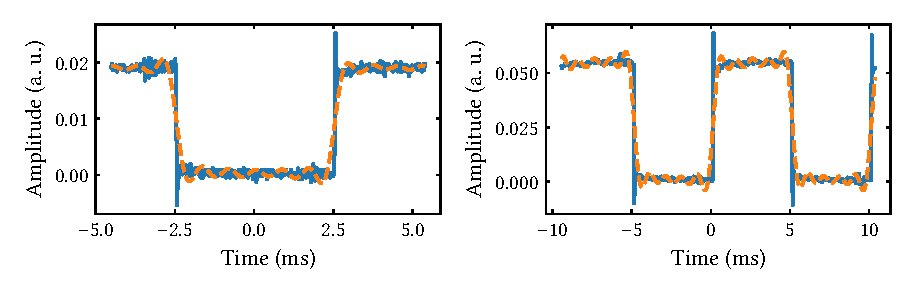
\includegraphics{figures/eom_extinction_155.pdf}
}
\caption{Measurements of extinction ratio for \ac{rtp} (left) and \ac{bbo} (right). The dashed lines indicate the fourier series fit in order to find the high and low level of the signal. The results are $>108:1$ for \ac{rtp} and $>129:1$ for \ac{bbo}.}
\end{figure}
\todo{make plot nicer}


As the pockels cell will be used in the chopping, which currently has a frequency of $\SI{1.4}{\mega\hertz}$, limits for the repetition rate of the \acp{eom} were tested. During this process, it was noted that the amplitude of the signal from the pockels cell was incosistent and in fact, changed depending on the repetition rate. This was most notable in the \ac{rtp} crystal. To quantize this in more detail, a program was written, that ramped the repetition rate up in $\SI{60}{\second}$ intervals, after which the resulting signal was recorded and the amplitude evaluated. This results in the diagram shown in Figure~\ref{fig:eom_amp_time}, however it needs to be noted, that alternating voltages were applied to the pockels cell, contrary to the argument before. This was found simply, because the behaviour was worse if only one type of voltage was applied. The diagram clearly shows resonant-like behaviour for \ac{rtp}. This means, that in the future, the chopping will have to be done around $\SI{1.5}{\mega\hertz}$, where the amplitude of the signal is close to the maximum and therefore loss of laser power is mostly only insertion loss into the \ac{eom}.

\begin{figure}[t]
\label{fig:eom_amp_time}
\centering{
	\setlength{\figureheight}{2in}
	\setlength{\figurewidth}{\textwidth-1.2em}
	%% This file was created by tikzplotlib v0.9.4.
\begin{tikzpicture}

\definecolor{color0}{rgb}{0.12156862745098,0.466666666666667,0.705882352941177}
\definecolor{color1}{rgb}{1,0.498039215686275,0.0549019607843137}

\begin{axis}[
height=\figureheight,
minor xtick={},
minor ytick={},
scaled y ticks=false,
tick align=inside,
tick pos=both,
width=\figurewidth,
x grid style={white!69.0196078431373!black},
xlabel={Frequency (MHz)},
xmin=0.95, xmax=2.05,
xtick style={color=black},
xtick={0.8,1,1.2,1.4,1.6,1.8,2,2.2},
xticklabels={0.8,1.0,1.2,1.4,1.6,1.8,2.0,2.2},
y grid style={white!69.0196078431373!black},
y tick label style={/pgf/number format/fixed},
ylabel style={align=center},
ylabel={Normalized Amplitude},
ymin=-0.05, ymax=1.05,
ytick style={color=black},
ytick={-0.5,0,0.5,1,1.5},
yticklabels={−0.25,0.00,0.25,0.50,0.75}
]
\addplot [line width=1.5pt, color0]
table {%
1 0.958240471323278
1.00150075037519 0.955765591308188
1.00300150075038 0.955620537636412
1.00450225112556 0.957828600953296
1.00600300150075 0.960057446813028
1.00750375187594 0.959368323428149
1.00900450225113 0.95973152643672
1.01050525262631 0.958514421315365
1.0120060030015 0.955752982242716
1.01350675337669 0.959026147379477
1.01500750375188 0.957330048117813
1.01650825412706 0.955517438464046
1.01800900450225 0.958426138172206
1.01950975487744 0.960184432072817
1.02101050525263 0.954662718807043
1.02251125562781 0.958016651327419
1.024012006003 0.956794640653859
1.02551275637819 0.95670292248929
1.02701350675338 0.958396413490181
1.02851425712856 0.958777565962598
1.03001500750375 0.960395087416408
1.03151575787894 0.957947813665374
1.03301650825413 0.958031323565406
1.03451725862931 0.956163061821321
1.0360180090045 0.955926791211139
1.03751875937969 0.958272986056345
1.03901950975488 0.95505170622911
1.04052026013006 0.960819052702023
1.04202101050525 0.959326686521515
1.04352176088044 0.95976386574891
1.04502251125563 0.95656579400304
1.04652326163082 0.956506015665391
1.048024012006 0.955308766914294
1.04952476238119 0.959407919193947
1.05102551275638 0.960041499202804
1.05252626313157 0.962095161245471
1.05402701350675 0.960342333824507
1.05552776388194 0.957533571400656
1.05702851425713 0.957045323639139
1.05852926463232 0.9591802590765
1.0600300150075 0.960390880039044
1.06153076538269 0.959288110059708
1.06303151575788 0.959103380240884
1.06453226613307 0.953323553195595
1.06603301650825 0.955807451034018
1.06753376688344 0.958611700494804
1.06903451725863 0.957475113023956
1.07053526763382 0.95712458529806
1.072036018009 0.952163214985017
1.07353676838419 0.946277536130315
1.07503751875938 0.949171437518897
1.07653826913457 0.948656191005031
1.07803901950975 0.950590461355813
1.07953976988494 0.95302736113175
1.08104052026013 0.94981283982246
1.08254127063532 0.94967129521469
1.08404202101051 0.951560196282567
1.08554277138569 0.947497202737719
1.08704352176088 0.948292267303944
1.08854427213607 0.953492454767396
1.09004502251126 0.951033810050398
1.09154577288644 0.950733900735913
1.09304652326163 0.954660445426587
1.09454727363682 0.952588845485224
1.09604802401201 0.950605670921092
1.09754877438719 0.950589901252007
1.09904952476238 0.953635044910631
1.10055027513757 0.956073323957815
1.10205102551276 0.952880876144935
1.10355177588794 0.95136381505861
1.10505252626313 0.955331200231453
1.10655327663832 0.955772522423534
1.10805402701351 0.954588983710219
1.10955477738869 0.955208122295766
1.11105552776388 0.954974040511398
1.11255627813907 0.95533889688093
1.11405702851426 0.955810346033623
1.11555777888944 0.954486448243219
1.11705852926463 0.957977072857676
1.11855927963982 0.957009784362125
1.12006003001501 0.957671084729791
1.1215607803902 0.956120697539119
1.12306153076538 0.954364877548246
1.12456228114057 0.956276589227362
1.12606303151576 0.956856738236108
1.12756378189095 0.957991309705294
1.12906453226613 0.958389242089793
1.13056528264132 0.961176891030128
1.13206603301651 0.957751463767166
1.1335667833917 0.957958584409856
1.13506753376688 0.953271746107741
1.13656828414207 0.956289672764335
1.13806903451726 0.95944429298193
1.13956978489245 0.958053851023294
1.14107053526763 0.957840229352852
1.14257128564282 0.958198852288613
1.14407203601801 0.956483456269557
1.1455727863932 0.954099847810489
1.14707353676838 0.954562704188519
1.14857428714357 0.958692727512999
1.15007503751876 0.956410143134529
1.15157578789395 0.957657648149217
1.15307653826913 0.956547981849511
1.15457728864432 0.958266395851038
1.15607803901951 0.957129382470627
1.1575787893947 0.957728395804048
1.15907953976988 0.958627278470489
1.16058029014507 0.957657172316722
1.16208104052026 0.958501280060365
1.16358179089545 0.959253153993166
1.16508254127064 0.954479931414179
1.16658329164582 0.958137350018109
1.16808404202101 0.961062253868861
1.1695847923962 0.959097973263758
1.17108554277139 0.958039949668083
1.17258629314657 0.957680034998663
1.17408704352176 0.952280669679428
1.17558779389695 0.958389198358536
1.17708854427214 0.960630696934947
1.17858929464732 0.962576619772016
1.18009004502251 0.959731064035448
1.1815907953977 0.962578459193511
1.18309154577289 0.958544333871073
1.18459229614807 0.958373426654759
1.18609304652326 0.957629146927843
1.18759379689845 0.959584391626377
1.18909454727364 0.958749226461126
1.19059529764882 0.959207070091998
1.19209604802401 0.95989543903368
1.1935967983992 0.961934385675639
1.19509754877439 0.958192531512004
1.19659829914957 0.959751095065762
1.19809904952476 0.960051806117197
1.19959979989995 0.958903053903419
1.20110055027514 0.955628437309198
1.20260130065033 0.957119298503051
1.20410205102551 0.958244498426101
1.2056028014007 0.956584959012953
1.20710355177589 0.957344746487443
1.20860430215108 0.95768714594959
1.21010505252626 0.958072798078421
1.21160580290145 0.956623191320148
1.21310655327664 0.954999299973142
1.21460730365183 0.95358159630967
1.21610805402701 0.956368787927726
1.2176088044022 0.959661381757854
1.21910955477739 0.961160175498501
1.22061030515258 0.957436915242769
1.22211105552776 0.95778347553089
1.22361180590295 0.955564190303698
1.22511255627814 0.956049878384048
1.22661330665333 0.957914339275964
1.22811405702851 0.962212982193289
1.2296148074037 0.962027724779185
1.23111555777889 0.95912236113418
1.23261630815408 0.960104359660653
1.23411705852926 0.957928486854394
1.23561780890445 0.958254466997473
1.23711855927964 0.960080482343446
1.23861930965483 0.961406140499506
1.24012006003002 0.961335550159664
1.2416208104052 0.961442835343715
1.24312156078039 0.962362636689688
1.24462231115558 0.960795793663401
1.24612306153077 0.961650062388667
1.24762381190595 0.964338435644848
1.24912456228114 0.963185505489029
1.25062531265633 0.960540447839679
1.25212606303152 0.961156260966209
1.2536268134067 0.962609595170174
1.25512756378189 0.963182097882494
1.25662831415708 0.960715501104284
1.25812906453227 0.96239829298671
1.25962981490745 0.959605499852459
1.26113056528264 0.959805522464988
1.26263131565783 0.961463234079288
1.26413206603302 0.960663753574888
1.2656328164082 0.962973275813607
1.26713356678339 0.963290504535161
1.26863431715858 0.964067749651528
1.27013506753377 0.962768609978102
1.27163581790895 0.962032074797884
1.27313656828414 0.962159288082527
1.27463731865933 0.961315857572643
1.27613806903452 0.959632331053591
1.2776388194097 0.965045026781337
1.27913956978489 0.965489490039274
1.28064032016008 0.963041516981085
1.28214107053527 0.962760921659839
1.28364182091046 0.958783219042116
1.28514257128564 0.956806426778895
1.28664332166083 0.961272700023716
1.28814407203602 0.963483274658152
1.28964482241121 0.960101349370105
1.29114557278639 0.963041566088618
1.29264632316158 0.962197027825909
1.29414707353677 0.957666906132081
1.29564782391196 0.955889834304999
1.29714857428714 0.958587609982291
1.29864932466233 0.959524842114937
1.30015007503752 0.96214740642688
1.30165082541271 0.961492015830745
1.30315157578789 0.961430465687755
1.30465232616308 0.95985819063399
1.30615307653827 0.960090913897877
1.30765382691346 0.960375844331188
1.30915457728864 0.960109805015276
1.31065532766383 0.959085540706062
1.31215607803902 0.9569463603454
1.31365682841421 0.9579875593595
1.31515757878939 0.95611309300985
1.31665832916458 0.960491358134389
1.31815907953977 0.95872128728402
1.31965982991496 0.955977555934172
1.32116058029015 0.958420576375087
1.32266133066533 0.957716812759288
1.32416208104052 0.957653024372643
1.32566283141571 0.95832384996544
1.3271635817909 0.957258009179264
1.32866433216608 0.961863870117037
1.33016508254127 0.956297786430208
1.33166583291646 0.957938412598544
1.33316658329165 0.95612214422965
1.33466733366683 0.956387418251376
1.33616808404202 0.958510151957272
1.33766883441721 0.956674669730271
1.3391695847924 0.958546829715016
1.34067033516758 0.958088160393557
1.34217108554277 0.959642365940971
1.34367183591796 0.956764404422306
1.34517258629315 0.955471238059799
1.34667333666833 0.956593056180324
1.34817408704352 0.957225551293764
1.34967483741871 0.958430846998295
1.3511755877939 0.957182469951054
1.35267633816908 0.959033135417604
1.35417708854427 0.957172501680379
1.35567783891946 0.953821687695856
1.35717858929465 0.955945938027054
1.35867933966983 0.955772774384042
1.36018009004502 0.954206314700641
1.36168084042021 0.947928941083229
1.3631815907954 0.950364385855713
1.36468234117059 0.943945314088795
1.36618309154577 0.946026004521651
1.36768384192096 0.946444065763184
1.36918459229615 0.948300281655659
1.37068534267134 0.947472285027374
1.37218609304652 0.945797086812219
1.37368684342171 0.946190842731405
1.3751875937969 0.950208072194968
1.37668834417209 0.945957627255254
1.37818909454727 0.9500503612302
1.37968984492246 0.953496310358774
1.38119059529765 0.947551644686542
1.38269134567284 0.948940501056929
1.38419209604802 0.946486025407657
1.38569284642321 0.948471267937629
1.3871935967984 0.948269822920463
1.38869434717359 0.951443393318912
1.39019509754877 0.952586121570915
1.39169584792396 0.953770132477949
1.39319659829915 0.952490808219111
1.39469734867434 0.94948760728426
1.39619809904952 0.953849403328844
1.39769884942471 0.955550001388454
1.3991995997999 0.956871208879841
1.40070035017509 0.958575920687336
1.40220110055028 0.956872617491259
1.40370185092546 0.955912129191621
1.40520260130065 0.9572639097938
1.40670335167584 0.957065816362467
1.40820410205103 0.956459636487517
1.40970485242621 0.962231302654412
1.4112056028014 0.964475531265138
1.41270635317659 0.967007482884559
1.41420710355178 0.966360777644639
1.41570785392696 0.967952132814654
1.41720860430215 0.969136112335762
1.41870935467734 0.973200131152582
1.42021010505253 0.972649782528349
1.42171085542771 0.976632744213351
1.4232116058029 0.979069938736645
1.42471235617809 0.979046443468039
1.42621310655328 0.982522949054918
1.42771385692846 0.985903499164381
1.42921460730365 0.986550008150956
1.43071535767884 0.984116777042617
1.43221610805403 0.981710005367905
1.43371685842921 0.983203743188068
1.4352176088044 0.982672700419196
1.43671835917959 0.985848484768294
1.43821910955478 0.985887003084258
1.43971985992996 0.986685464673487
1.44122061030515 0.986511748438456
1.44272136068034 0.988519686926714
1.44422211105553 0.986595920148964
1.44572286143072 0.988575389019042
1.4472236118059 0.99223149423754
1.44872436218109 0.990482961004897
1.45022511255628 0.993030508205783
1.45172586293147 0.992867755539669
1.45322661330665 0.991973576332518
1.45472736368184 0.993130362708759
1.45622811405703 0.993570902991989
1.45772886443222 0.991406769194645
1.4592296148074 0.993541328296636
1.46073036518259 0.992447970693333
1.46223111555778 0.991777585813055
1.46373186593297 0.992910829122715
1.46523261630815 0.990141709586069
1.46673336668334 0.996490133472951
1.46823411705853 0.993793567196568
1.46973486743372 0.993975759061437
1.4712356178089 0.990760536515173
1.47273636818409 0.993434517102197
1.47423711855928 0.99289138585418
1.47573786893447 0.992671538950003
1.47723861930965 0.995148596857487
1.47873936968484 0.994834128642621
1.48024012006003 0.992557123565414
1.48174087043522 0.990966484801331
1.48324162081041 0.986709826611075
1.48474237118559 0.986202516001605
1.48624312156078 0.992434236930288
1.48774387193597 0.990935890404871
1.48924462231116 0.991597080075278
1.49074537268634 0.990332267594491
1.49224612306153 0.990528329630221
1.49374687343672 0.983983867435916
1.49524762381191 0.984055294234496
1.49674837418709 0.987046901759671
1.49824912456228 0.985227123886383
1.49974987493747 0.984950118247705
1.50125062531266 0.983554141503584
1.50275137568784 0.988903688962851
1.50425212606303 0.987908561232092
1.50575287643822 0.986341633213486
1.50725362681341 0.985817989471691
1.50875437718859 0.984329039049079
1.51025512756378 0.984039899053588
1.51175587793897 0.980797323741189
1.51325662831416 0.984920726566432
1.51475737868934 0.988387553183224
1.51625812906453 0.990727096830401
1.51775887943972 0.987615583712499
1.51925962981491 0.98849995620113
1.5207603801901 0.985477848887382
1.52226113056528 0.984773131620957
1.52376188094047 0.984956455521953
1.52526263131566 0.983814528111015
1.52676338169085 0.987561500748046
1.52826413206603 0.988246278716138
1.52976488244122 0.9904443961726
1.53126563281641 0.99127853973567
1.5327663831916 0.988998470406475
1.53426713356678 0.990083282493234
1.53576788394197 0.994369210791513
1.53726863431716 0.992619476982356
1.53876938469235 0.991015637903889
1.54027013506753 0.992285297017221
1.54177088544272 0.994098982779349
1.54327163581791 0.99035062551897
1.5447723861931 0.989379013962044
1.54627313656828 0.993310328204182
1.54777388694347 0.993275437370949
1.54927463731866 0.994363777432792
1.55077538769385 0.994250417882373
1.55227613806903 0.99278444384898
1.55377688844422 0.995732364573626
1.55527763881941 0.99359212566352
1.5567783891946 0.991901723559053
1.55827913956978 0.993889892834922
1.55977988994497 0.990493289886479
1.56128064032016 0.993969635878333
1.56278139069535 0.991296387426684
1.56428214107054 0.993083108098569
1.56578289144572 0.995772104621653
1.56728364182091 0.990401706508612
1.5687843921961 0.989657798171885
1.57028514257129 0.989986878225522
1.57178589294647 0.991666505587868
1.57328664332166 0.991071810451643
1.57478739369685 0.992223717750986
1.57628814407204 0.992549585159107
1.57778889444722 0.990013428549714
1.57928964482241 0.991047133425429
1.5807903951976 0.99050473153248
1.58229114557279 0.989318097686439
1.58379189594797 0.989273362791115
1.58529264632316 0.989755700151416
1.58679339669835 0.990023368705132
1.58829414707354 0.993213724730029
1.58979489744872 0.991655209783005
1.59129564782391 0.992961675655285
1.5927963981991 0.990920435841857
1.59429714857429 0.988655599433433
1.59579789894947 0.990049787131169
1.59729864932466 0.992187528822471
1.59879939969985 0.992668270586837
1.60030015007504 0.990006746239323
1.60180090045023 0.99149341229318
1.60330165082541 0.993434857951524
1.6048024012006 0.989969360795772
1.60630315157579 0.993995584222323
1.60780390195098 0.993208356770707
1.60930465232616 0.991625669940365
1.61080540270135 0.992188752745079
1.61230615307654 0.993857819864978
1.61380690345173 0.992056827268176
1.61530765382691 0.993192173298398
1.6168084042021 0.991838747576879
1.61830915457729 0.992656107680591
1.61980990495248 0.992310649103638
1.62131065532766 0.991234780869187
1.62281140570285 0.990188597702586
1.62431215607804 0.991068258475609
1.62581290645323 0.991800810878989
1.62731365682841 0.993812383002499
1.6288144072036 0.993723345731096
1.63031515757879 0.993561794553363
1.63181590795398 0.992466763132866
1.63331665832916 0.990707773412822
1.63481740870435 0.988979865764416
1.63631815907954 0.992521594377859
1.63781890945473 0.993645387297109
1.63931965982992 0.99454633434849
1.6408204102051 0.993176309646147
1.64232116058029 0.993146089806076
1.64382191095548 0.989623831163586
1.64532266133067 0.992017420393791
1.64682341170585 0.992402388732625
1.64832416208104 0.993118390394842
1.64982491245623 0.991798124216472
1.65132566283142 0.993130933841988
1.6528264132066 0.990642621254708
1.65432716358179 0.988569681120131
1.65582791395698 0.99052561434468
1.65732866433217 0.990243669764503
1.65882941470735 0.991531108094546
1.66033016508254 0.990741316328116
1.66183091545773 0.991546556117336
1.66333166583292 0.990913461501632
1.6648324162081 0.99091878479455
1.66633316658329 0.992187813941301
1.66783391695848 0.989528243669761
1.66933466733367 0.989674054650117
1.67083541770885 0.991045179257104
1.67233616808404 0.993784556325578
1.67383691845923 0.991686731938808
1.67533766883442 0.992384061456807
1.6768384192096 0.993961301148348
1.67833916958479 0.994910763725002
1.67983991995998 0.991823269217379
1.68134067033517 0.990551242000176
1.68284142071036 0.987716547309656
1.68434217108554 0.988031296125614
1.68584292146073 0.989176159731423
1.68734367183592 0.989322349250339
1.68884442221111 0.992472136819396
1.69034517258629 0.988281697615522
1.69184592296148 0.987333416458082
1.69334667333667 0.987806058992647
1.69484742371186 0.986714186428858
1.69634817408704 0.985358839750947
1.69784892446223 0.989069175546103
1.69934967483742 0.986222791398285
1.70085042521261 0.988609160693915
1.70235117558779 0.990861535217178
1.70385192596298 0.987439336070248
1.70535267633817 0.989357565379946
1.70685342671336 0.989473999668822
1.70835417708854 0.987571623086012
1.70985492746373 0.988004681713645
1.71135567783892 0.987529113088418
1.71285642821411 0.986038017008698
1.71435717858929 0.988675488346587
1.71585792896448 0.988771267922166
1.71735867933967 0.989729491866053
1.71885942971486 0.985587199779856
1.72036018009004 0.990017672176808
1.72186093046523 0.989616207359506
1.72336168084042 0.987190687150512
1.72486243121561 0.988534284750376
1.7263631815908 0.989932822349606
1.72786393196598 0.992437834512839
1.72936468234117 0.9862635627999
1.73086543271636 0.987599572946799
1.73236618309155 0.989514961623071
1.73386693346673 0.986403804106017
1.73536768384192 0.989220574191568
1.73686843421711 0.989474903526472
1.7383691845923 0.988704525396514
1.73986993496748 0.989507788622025
1.74137068534267 0.987890743026496
1.74287143571786 0.985234818501075
1.74437218609305 0.987014020571414
1.74587293646823 0.985811124601845
1.74737368684342 0.990443751317789
1.74887443721861 0.987022857165859
1.7503751875938 0.989605250196685
1.75187593796898 0.988998719016148
1.75337668834417 0.987638465035079
1.75487743871936 0.98670135549284
1.75637818909455 0.987379147239732
1.75787893946973 0.988740571030031
1.75937968984492 0.990153376343465
1.76088044022011 0.986757183863408
1.7623811905953 0.988944785801751
1.76388194097049 0.987147090573738
1.76538269134567 0.99145815331793
1.76688344172086 0.988606089778493
1.76838419209605 0.986640604468314
1.76988494247124 0.987865306132559
1.77138569284642 0.985823588067675
1.77288644322161 0.987532067195985
1.7743871935968 0.985685577343536
1.77588794397199 0.993161783876756
1.77738869434717 0.991185372304302
1.77888944472236 0.990391189705593
1.78039019509755 0.98861879173927
1.78189094547274 0.986965536633559
1.78339169584792 0.988488654778697
1.78489244622311 0.98793528876268
1.7863931965983 0.989626983631708
1.78789394697349 0.989111592782198
1.78939469734867 0.990455018837756
1.79089544772386 0.990158234332554
1.79239619809905 0.989403368087167
1.79389694847424 0.987168152227972
1.79539769884942 0.989473723774089
1.79689844922461 0.989103351605557
1.7983991995998 0.989499997376921
1.79989994997499 0.988820871406954
1.80140070035018 0.990017514164028
1.80290145072536 0.989269542050518
1.80440220110055 0.98807200694807
1.80590295147574 0.98846781835136
1.80740370185093 0.989774623821575
1.80890445222611 0.991132759321054
1.8104052026013 0.992358970655786
1.81190595297649 0.993543170240029
1.81340670335168 0.991902109538031
1.81490745372686 0.991993535596188
1.81640820410205 0.992391008200563
1.81790895447724 0.992050286365176
1.81940970485243 0.991080570931894
1.82091045522761 0.988241609196094
1.8224112056028 0.990260617734378
1.82391195597799 0.986822492944435
1.82541270635318 0.99051863017716
1.82691345672836 0.994361878070481
1.82841420710355 0.99101031557246
1.82991495747874 0.989096502920396
1.83141570785393 0.987801845470019
1.83291645822911 0.988987155653354
1.8344172086043 0.989670221778665
1.83591795897949 0.991632957298819
1.83741870935468 0.990515669659922
1.83891945972987 0.991726421242308
1.84042021010505 0.989990370283697
1.84192096048024 0.990689934140664
1.84342171085543 0.989166323038494
1.84492246123062 0.989715805260962
1.8464232116058 0.991476875418131
1.84792396198099 0.991443523749963
1.84942471235618 0.990505441374355
1.85092546273137 0.991803433087078
1.85242621310655 0.992164897841376
1.85392696348174 0.98913469397926
1.85542771385693 0.989289872176304
1.85692846423212 0.992038341063532
1.8584292146073 0.992300539640784
1.85992996498249 0.991907011969771
1.86143071535768 0.991109597573001
1.86293146573287 0.99128146149641
1.86443221610805 0.991297854181849
1.86593296648324 0.992186853608812
1.86743371685843 0.993232421759511
1.86893446723362 0.990526082426639
1.8704352176088 0.98954470610329
1.87193596798399 0.990218493899296
1.87343671835918 0.991260232871402
1.87493746873437 0.993875686400055
1.87643821910955 0.994551413037214
1.87793896948474 0.994768072631052
1.87943971985993 0.992066330576104
1.88094047023512 0.989808259157793
1.88244122061031 0.989762630581066
1.88394197098549 0.9910037778338
1.88544272136068 0.992162489657275
1.88694347173587 0.992096880758961
1.88844422211106 0.99385121817957
1.88994497248624 0.992729177154223
1.89144572286143 0.993282155631064
1.89294647323662 0.991137924754717
1.89444722361181 0.992584939285654
1.89594797398699 0.992517150870396
1.89744872436218 0.995666245372067
1.89894947473737 0.992885105219143
1.90045022511256 0.996243427342429
1.90195097548774 0.992511855690603
1.90345172586293 0.990671683010141
1.90495247623812 0.993967029334798
1.90645322661331 0.99131248559687
1.90795397698849 0.990794501863476
1.90945472736368 0.991229524726672
1.91095547773887 0.987714997944258
1.91245622811406 0.988693151746873
1.91395697848924 0.99094066262149
1.91545772886443 0.990793821461196
1.91695847923962 0.991925309729863
1.91845922961481 0.994522808768912
1.91995997998999 0.994062450808532
1.92146073036518 0.995803472256004
1.92296148074037 0.993417553498957
1.92446223111556 0.994632714007127
1.92596298149075 0.998057456033245
1.92746373186593 0.996688863782786
1.92896448224112 0.997499360718917
1.93046523261631 0.995856506166173
1.9319659829915 0.995068798839263
1.93346673336668 0.994084965277339
1.93496748374187 0.999138616034683
1.93646823411706 0.997963892786656
1.93796898449225 0.995535139548336
1.93946973486743 0.99725340801629
1.94097048524262 0.995547610713072
1.94247123561781 0.995898032703005
1.943971985993 0.994897580668802
1.94547273636818 0.994170439436946
1.94697348674337 0.997196837541095
1.94847423711856 0.996607279482769
1.94997498749375 0.999020634622417
1.95147573786893 0.997984933055679
1.95297648824412 0.996352996216267
1.95447723861931 0.996090309084277
1.9559779889945 0.99750199313539
1.95747873936968 0.996219632786986
1.95897948974487 0.994248897487255
1.96048024012006 0.995737050884722
1.96198099049525 0.994353850215428
1.96348174087044 0.995232421224981
1.96498249124562 0.995260767727472
1.96648324162081 0.996778323406204
1.967983991996 0.995551313018955
1.96948474237119 0.995070637538261
1.97098549274637 0.997447641273714
1.97248624312156 0.995418494668022
1.97398699349675 0.998135493735855
1.97548774387194 0.996117364222715
1.97698849424712 1
1.97848924462231 0.995723892919332
1.9799899949975 0.995987409796398
1.98149074537269 0.996536027996938
1.98299149574787 0.995718812461595
1.98449224612306 0.99827548498243
1.98599299649825 0.998300865400035
1.98749374687344 0.99549734164138
1.98899449724862 0.998375792182429
1.99049524762381 0.998213715956604
1.991995997999 0.998644041407232
1.99349674837419 0.995064728145437
1.99499749874937 0.998729582407633
1.99649824912456 0.995691058325329
1.99799899949975 0.997729817549313
1.99949974987494 0.998318544970013
};
\addplot [line width=1.5pt, color1]
table {%
1 0.990147522249168
1.00200400801603 0.996449250342955
1.00400801603206 1
1.0060120240481 0.9963419962043
1.00801603206413 0.988784977607459
1.01002004008016 0.980377322351208
1.01202404809619 0.974915985705703
1.01402805611222 0.967795520260504
1.01603206412826 0.970933375870833
1.01803607214429 0.973807283028414
1.02004008016032 0.977437369528237
1.02204408817635 0.976173268800942
1.02404809619238 0.972605113172264
1.02605210420842 0.974057022805923
1.02805611222445 0.976222416906075
1.03006012024048 0.978243551923738
1.03206412825651 0.977373109318136
1.03406813627255 0.973573550719129
1.03607214428858 0.964712775672747
1.03807615230461 0.956161333998036
1.04008016032064 0.934348951680696
1.04208416833667 0.91177915371219
1.04408817635271 0.909922460683172
1.04609218436874 0.90746325473495
1.04809619238477 0.904622874181154
1.0501002004008 0.894689952649373
1.05210420841683 0.889925334656508
1.05410821643287 0.903019231383528
1.0561122244489 0.917011018066523
1.05811623246493 0.91974099343212
1.06012024048096 0.924971027654564
1.06212424849699 0.916205553422628
1.06412825651303 0.904728948993425
1.06613226452906 0.900693365866258
1.06813627254509 0.903466819453237
1.07014028056112 0.898393840189015
1.07214428857715 0.887114074277531
1.07414829659319 0.881777650745441
1.07615230460922 0.886922818723089
1.07815631262525 0.894338867208478
1.08016032064128 0.906320982658451
1.08216432865731 0.911276905433844
1.08416833667335 0.914898614838391
1.08617234468938 0.913739517762913
1.08817635270541 0.917380036117783
1.09018036072144 0.918226265428739
1.09218436873748 0.925693597841367
1.09418837675351 0.928724689372379
1.09619238476954 0.92882735228527
1.09819639278557 0.930270621931059
1.1002004008016 0.932014646270108
1.10220440881764 0.928902212971339
1.10420841683367 0.930286187713311
1.1062124248497 0.931473521744415
1.10821643286573 0.933899709954273
1.11022044088176 0.93536994767931
1.1122244488978 0.93987338566696
1.11422845691383 0.946606382936369
1.11623246492986 0.955821374499782
1.11823647294589 0.960972196951436
1.12024048096192 0.970306810784943
1.12224448897796 0.978628055435876
1.12424849699399 0.983176179823504
1.12625250501002 0.990113457820024
1.12825651302605 0.994696458939781
1.13026052104208 0.991588341086651
1.13226452905812 0.99320825578575
1.13426853707415 0.987287284711055
1.13627254509018 0.982665312920143
1.13827655310621 0.975266382570401
1.14028056112224 0.960237099610991
1.14228456913828 0.956485255019735
1.14428857715431 0.961944846813158
1.14629258517034 0.965367987320258
1.14829659318637 0.967590559790251
1.1503006012024 0.968771128746347
1.15230460921844 0.968417573218284
1.15430861723447 0.971329466211875
1.1563126252505 0.974885802191193
1.15831663326653 0.97778092328156
1.16032064128257 0.980006725851132
1.1623246492986 0.984025534233995
1.16432865731463 0.981168445752826
1.16633266533066 0.986217389021952
1.16833667334669 0.990800898510473
1.17034068136273 0.991436596124322
1.17234468937876 0.991964682218703
1.17434869739479 0.992056879945657
1.17635270541082 0.990752566956474
1.17835671342685 0.990742879528281
1.18036072144289 0.982637915602529
1.18236472945892 0.969185524605911
1.18436873747495 0.958581894316526
1.18637274549098 0.95442273383677
1.18837675350701 0.949738199489497
1.19038076152305 0.944185235319689
1.19238476953908 0.938651704715228
1.19438877755511 0.934774542307002
1.19639278557114 0.929027077313301
1.19839679358717 0.922922130085649
1.20040080160321 0.922676080722958
1.20240480961924 0.935078428313042
1.20440881763527 0.942296467728409
1.2064128256513 0.947631909221674
1.20841683366733 0.951268047196897
1.21042084168337 0.953509542081908
1.2124248496994 0.955890027435991
1.21442885771543 0.954931134481887
1.21643286573146 0.950721784380327
1.21843687374749 0.942891167365624
1.22044088176353 0.933158497307502
1.22244488977956 0.918317351727589
1.22444889779559 0.910525193822782
1.22645290581162 0.906345556709246
1.22845691382766 0.907996797176429
1.23046092184369 0.912328509096334
1.23246492985972 0.913972865721103
1.23446893787575 0.910332353605415
1.23647294589178 0.89340234592896
1.23847695390782 0.865940331691956
1.24048096192385 0.859778480175663
1.24248496993988 0.849900288412112
1.24448897795591 0.841286524781878
1.24649298597194 0.829242084818544
1.24849699398798 0.820813125646135
1.25050100200401 0.817703503226655
1.25250501002004 0.801065230577676
1.25450901803607 0.774298150788868
1.2565130260521 0.740453496437832
1.25851703406814 0.739954065191943
1.26052104208417 0.76767533931526
1.2625250501002 0.791017602344053
1.26452905811623 0.778210564475428
1.26653306613226 0.771581372907181
1.2685370741483 0.762572688193442
1.27054108216433 0.75013613220831
1.27254509018036 0.758522945219106
1.27454909819639 0.788287847089672
1.27655310621242 0.81756306493414
1.27855711422846 0.840154742533852
1.28056112224449 0.858278127024254
1.28256513026052 0.852683785489505
1.28456913827655 0.847977161563038
1.28657314629259 0.850513859874316
1.28857715430862 0.860042269301684
1.29058116232465 0.870581622668319
1.29258517034068 0.877856486579903
1.29458917835671 0.875979628136906
1.29659318637275 0.863840417538519
1.29859719438878 0.836729652883377
1.30060120240481 0.801306391636757
1.30260521042084 0.762509918091199
1.30460921843687 0.730006136659631
1.30661322645291 0.728001598736697
1.30861723446894 0.736030586415814
1.31062124248497 0.742470552940228
1.312625250501 0.749113799947671
1.31462925851703 0.759293008523048
1.31663326653307 0.772488286503453
1.3186372745491 0.777783381402752
1.32064128256513 0.768202761355657
1.32264529058116 0.767083929092863
1.32464929859719 0.756776407361932
1.32665330661323 0.734596921476218
1.32865731462926 0.70621156766449
1.33066132264529 0.658515826160761
1.33266533066132 0.584512115112871
1.33466933867735 0.451560407871815
1.33667334669339 0.268801347469669
1.33867735470942 0.1013779676603
1.34068136272545 0.0129681528116031
1.34268537074148 0.00535405274501119
1.34468937875751 0.0248866288159281
1.34669338677355 0.0710103357231658
1.34869739478958 0.120421948269728
1.35070140280561 0.177259049051772
1.35270541082164 0.232553624031913
1.35470941883768 0.289235273107845
1.35671342685371 0.33657674608237
1.35871743486974 0.380751255940646
1.36072144288577 0.41963856191516
1.3627254509018 0.452494293591471
1.36472945891784 0.453663786635154
1.36673346693387 0.447677849601862
1.3687374749499 0.439902936496915
1.37074148296593 0.435169329921563
1.37274549098196 0.426723966753527
1.374749498998 0.409529577073103
1.37675350701403 0.384249911201248
1.37875751503006 0.364662930017059
1.38076152304609 0.379935573008099
1.38276553106212 0.417923116634041
1.38476953907816 0.466802900908619
1.38677354709419 0.514627437920525
1.38877755511022 0.550233601098406
1.39078156312625 0.577830605665268
1.39278557114228 0.618404237161702
1.39478957915832 0.666337675529325
1.39679358717435 0.714776094474533
1.39879759519038 0.731576695007852
1.40080160320641 0.728695151297767
1.40280561122244 0.718581599848213
1.40480961923848 0.707713128867219
1.40681362725451 0.682929394587653
1.40881763527054 0.650632950688319
1.41082164328657 0.604392589802555
1.41282565130261 0.555719346569591
1.41482965931864 0.522738884530519
1.41683366733467 0.492954545629567
1.4188376753507 0.483430738270722
1.42084168336673 0.481803931684536
1.42284569138277 0.466504289008159
1.4248496993988 0.448438108584691
1.42685370741483 0.423732799525181
1.42885771543086 0.409284505603413
1.43086172344689 0.41068390859983
1.43286573146293 0.423369543218647
1.43486973947896 0.451973782893847
1.43687374749499 0.502907481274595
1.43887775551102 0.570343534701867
1.44088176352705 0.621245228335099
1.44288577154309 0.67035227261384
1.44488977955912 0.697581370990058
1.44689378757515 0.725155342377079
1.44889779559118 0.749573832926115
1.45090180360721 0.781453630117277
1.45290581162325 0.807411081409043
1.45490981963928 0.828769898198832
1.45691382765531 0.853021118580954
1.45891783567134 0.874130054410369
1.46092184368737 0.887268118233096
1.46292585170341 0.895439745342307
1.46492985971944 0.89865325107728
1.46693386773547 0.900682152620288
1.4689378757515 0.913208783228331
1.47094188376753 0.920556831364899
1.47294589178357 0.933831608325496
1.4749498997996 0.953901159656848
1.47695390781563 0.962187785787258
1.47895791583166 0.962660571902397
1.4809619238477 0.956822861381727
1.48296593186373 0.951286237530228
1.48496993987976 0.954113464530224
1.48697394789579 0.955667386038112
1.48897795591182 0.9620479196171
1.49098196392786 0.958983237106774
1.49298597194389 0.964482318954497
1.49498997995992 0.964718791377672
1.49699398797595 0.970971764357054
1.49899799599198 0.963911079252774
1.50100200400802 0.960189322260788
1.50300601202405 0.951526658241931
1.50501002004008 0.946413946639297
1.50701402805611 0.944226713135448
1.50901803607214 0.946212493434078
1.51102204408818 0.94361089018374
1.51302605210421 0.941759075612268
1.51503006012024 0.938934272795696
1.51703406813627 0.922356835443548
1.5190380761523 0.920126452695828
1.52104208416834 0.912802316898804
1.52304609218437 0.910326831856641
1.5250501002004 0.900646715467071
1.52705410821643 0.914683346800804
1.52905811623247 0.911438392305171
1.5310621242485 0.912515132833622
1.53306613226453 0.912552086881341
1.53507014028056 0.919593564854721
1.53707414829659 0.928978459781314
1.53907815631263 0.923024188710286
1.54108216432866 0.933691871253146
1.54308617234469 0.940488288877388
1.54509018036072 0.942430945217806
1.54709418837675 0.95313965555286
1.54909819639279 0.954562377867999
1.55110220440882 0.955867373730627
1.55310621242485 0.955652833016935
1.55511022044088 0.958146767095367
1.55711422845691 0.956376442220833
1.55911823647295 0.960313400172248
1.56112224448898 0.951010574779829
1.56312625250501 0.952584941471386
1.56513026052104 0.945455367079903
1.56713426853707 0.942151144143276
1.56913827655311 0.941928465735052
1.57114228456914 0.929156634192575
1.57314629258517 0.925163007080831
1.5751503006012 0.920241565858794
1.57715430861723 0.892679143478064
1.57915831663327 0.861437570119223
1.5811623246493 0.823742678293933
1.58316633266533 0.798335841336236
1.58517034068136 0.796509668933135
1.58717434869739 0.810099086404515
1.58917835671343 0.82036994310506
1.59118236472946 0.826653763018507
1.59318637274549 0.84857722606719
1.59519038076152 0.854635547758425
1.59719438877756 0.862181868975769
1.59919839679359 0.856311131293999
1.60120240480962 0.855347027707202
1.60320641282565 0.849017660830303
1.60521042084168 0.848677533814196
1.60721442885772 0.850313925170857
1.60921843687375 0.850846684287975
1.61122244488978 0.851090119749671
1.61322645290581 0.851154305896025
1.61523046092184 0.841953716516502
1.61723446893788 0.837055049909924
1.61923847695391 0.83590735059939
1.62124248496994 0.816294581942979
1.62324649298597 0.81095987775926
1.625250501002 0.804595423237099
1.62725450901804 0.797916608209712
1.62925851703407 0.790433521757317
1.6312625250501 0.803227084516205
1.63326653306613 0.832630187197973
1.63527054108216 0.85990570400783
1.6372745490982 0.890351180761593
1.63927855711423 0.90593814631326
1.64128256513026 0.90444758523621
1.64328657314629 0.910250959438529
1.64529058116232 0.901153145286245
1.64729458917836 0.895132936122115
1.64929859719439 0.881597789621585
1.65130260521042 0.879849280737131
1.65330661322645 0.87201353763268
1.65531062124249 0.862687612195622
1.65731462925852 0.842226672394332
1.65931863727455 0.813822625748024
1.66132264529058 0.821184720807375
1.66332665330661 0.826555093224279
1.66533066132265 0.824934132700503
1.66733466933868 0.824855910800204
1.66933867735471 0.829937536734838
1.67134268537074 0.820369038924808
1.67334669338677 0.808779283451578
1.67535070140281 0.792304342561603
1.67735470941884 0.794054632195295
1.67935871743487 0.798859828234182
1.6813627254509 0.811241341511729
1.68336673346693 0.808227818984318
1.68537074148297 0.803468091968238
1.687374749499 0.777619884722728
1.68937875751503 0.741087256945282
1.69138276553106 0.701997121053335
1.69338677354709 0.668973969608009
1.69539078156313 0.633122151293556
1.69739478957916 0.589316775354579
1.69939879759519 0.565248172149939
1.70140280561122 0.549264036470629
1.70340681362725 0.529929192518192
1.70541082164329 0.507552798987864
1.70741482965932 0.481883746478969
1.70941883767535 0.474531565385928
1.71142284569138 0.476572812173793
1.71342685370741 0.499931895254012
1.71543086172345 0.532134568214333
1.71743486973948 0.568555256848866
1.71943887775551 0.589685562253191
1.72144288577154 0.591015833223362
1.72344689378758 0.527412811427517
1.72545090180361 0.431830649374391
1.72745490981964 0.350900915074853
1.72945891783567 0.329661378178791
1.7314629258517 0.326837643187103
1.73346693386774 0.264939108328027
1.73547094188377 0.204826562254376
1.7374749498998 0.139972839614973
1.73947895791583 0.0339705076220396
1.74148296593186 0.0356423774200809
1.7434869739479 0.0572392212907274
1.74549098196393 0.0550751411090706
1.74749498997996 0.0461074215654644
1.74949899799599 0.0411860156350086
1.75150300601202 0.0392729633987682
1.75350701402806 0.0339988284154785
1.75551102204409 0.0268363619298178
1.75751503006012 0.0250819059755168
1.75951903807615 0.0311031805420922
1.76152304609218 0.0351605227207835
1.76352705410822 0.022549614958429
1.76553106212425 0.00290674894146167
1.76753507014028 0.01314539693774
1.76953907815631 0.0119826107479196
1.77154308617234 0.00290797930581336
1.77354709418838 0.00433344427781917
1.77555110220441 0.0083970086430005
1.77755511022044 0.0137226895229455
1.77955911823647 0.016757574417292
1.7815631262525 0.0160366803206256
1.78356713426854 0.0128143812696489
1.78557114228457 0.00930088892611756
1.7875751503006 0.00789618916116642
1.78957915831663 0.00677060476467479
1.79158316633267 0.0070292958723393
1.7935871743487 0.00730902731243552
1.79559118236473 0.00659004426938179
1.79759519038076 0.00528084695234535
1.79959919839679 0.00274241131111955
1.80160320641283 0.00138420395118155
1.80360721442886 0.000649030432795286
1.80561122244489 0.000424749540525694
1.80761523046092 0.000677187360382355
1.80961923847695 0.00102395195934837
1.81162324649299 0.00164658529242199
1.81362725450902 0.00171680747635963
1.81563126252505 0.00114819916379941
1.81763527054108 0.000301148037865478
1.81963927855711 0.000364653714987603
1.82164328657315 0.000603453552258338
1.82364729458918 0.000409588220666471
1.82565130260521 0.000375579255093681
1.82765531062124 0.000518662816592216
1.82965931863727 0.000371881105391446
1.83166332665331 0.000469535064475846
1.83366733466934 0.000287486972774001
1.83567134268537 0.000438564261961853
1.8376753507014 0.000567149742388533
1.83967935871743 0.000469395442449709
1.84168336673347 0.000558952135088967
1.8436873747495 0.00044054984011275
1.84569138276553 0.00050075958368147
1.84769539078156 0.000267459345130497
1.8496993987976 0.000495184332038404
1.85170340681363 0.000363573793251984
1.85370741482966 0.000394267764477301
1.85571142284569 0.000342026571219025
1.85771543086172 0.000387675434890925
1.85971943887776 0.000524700226956923
1.86172344689379 0.000395282647529134
1.86372745490982 0.000340664438623727
1.86573146292585 0.000243721640231764
1.86773547094188 0.000369947338612277
1.86973947895792 0.000450152494712604
1.87174348697395 0.000376344976983526
1.87374749498998 0.000376940036997563
1.87575150300601 0.000295597796783004
1.87775551102204 0.000331202357507041
1.87975951903808 0.000347906727388508
1.88176352705411 0.000435719180200661
1.88376753507014 0.00042423211237733
1.88577154308617 0.000310048927748007
1.8877755511022 0.000413917257459636
1.88977955911824 0.000362764218728939
1.89178356713427 0.000468114931343644
1.8937875751503 0.000557194453075756
1.89579158316633 0.000629474233453675
1.89779559118236 0.000799533959968154
1.8997995991984 0.00114583513514682
1.90180360721443 0.00149439698944496
1.90380761523046 0.00202001774870554
1.90581162324649 0.00287439502623656
1.90781563126252 0.00350310808217468
1.90981963927856 0.00411462938707015
1.91182364729459 0.00394291855588353
1.91382765531062 0.00292627338284999
1.91583166332665 0.00178147264287546
1.91783567134269 0.00087997539730436
1.91983967935872 0.000452339404519718
1.92184368737475 0.000667257315844623
1.92384769539078 0.000693613182914989
1.92585170340681 0.000706437925122319
1.92785571142285 0.000587846141545486
1.92985971943888 0.000555740416293483
1.93186372745491 0.00064842531605033
1.93386773547094 0.00107373798432945
1.93587174348697 0.00178317833824435
1.93787575150301 0.00232764565848849
1.93987975951904 0.00264467120041838
1.94188376753507 0.00217268250407233
1.9438877755511 0.00165840984093318
1.94589178356713 0.00120638414983723
1.94789579158317 0.000932379417200836
1.9498997995992 0.00118757992892196
1.95190380761523 0.00117424441237809
1.95390781563126 0.00122099728692654
1.95591182364729 0.00148623656772427
1.95791583166333 0.00229975273796449
1.95991983967936 0.00307884976018462
1.96192384769539 0.00353926573072403
1.96392785571142 0.00569118080607769
1.96593186372745 0.00631058717023708
1.96793587174349 0.00863325400897858
1.96993987975952 0.0112870517651339
1.97194388777555 0.0132916376879852
1.97394789579158 0.0150055096455665
1.97595190380762 0.0169971157246103
1.97795591182365 0.0202346560335841
1.97995991983968 0.0210070218711308
1.98196392785571 0.0237536061631987
1.98396793587174 0.0224867367923269
1.98597194388778 0.0210393258392585
1.98797595190381 0.0181491021939281
1.98997995991984 0.0122190390906775
1.99198396793587 0.00621081270727623
1.9939879759519 0.00209201550145104
1.99599198396794 0.0112711257752445
1.99799599198397 0.02314577557285
2 0.0384613383521769
};
\end{axis}

\end{tikzpicture}

	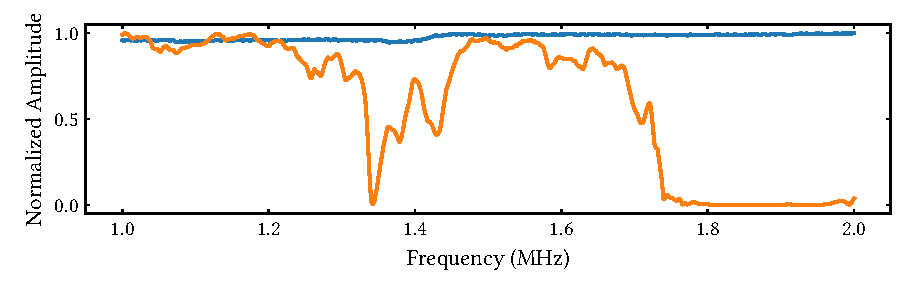
\includegraphics{figures/eom_amp_time_155.pdf}
}
\caption{Shown is the amplitude of a laser whose polarization was rotated by a pockels cell and then filtered using a polarizing beam splitter. The frequency is the repetition rate of the voltage placed into the \ac{eom}. The two materials are \ac{rtp} (orange) \ac{bbo} (blue). The curves are normalized to their maximum value.}
\end{figure}

